\section{Testy rozmytych regulatorów PID}
\label{lab:zad4}

W tym samym programie zaimplementowac rozmyty algorytm PI lub PID. Dla tej samej
trajektorii zmian sygnału wartosci zadanej spróbowac dobrac parametry lokalnych
algorytmów PI (PID) w taki sposób, aby osiagnac lepsza jakosc regulacji w porównaniu
z regulatorem klasycznym (pojedynczym). Wykonac eksperymenty dla 3 regulatorów
lokalnych. Omówic proces doboru parametrów i zamiescic uzyskane przebiegi regulacji.

\subsection{Funkcje przynależności}
\label{lab:zad4:fuzzyFunction}

\begin{figure}[H] 
    \centering
    % This file was created by matlab2tikz.
%
\definecolor{mycolor1}{rgb}{0.00000,0.44700,0.74100}%
\definecolor{mycolor2}{rgb}{0.85000,0.32500,0.09800}%
\definecolor{mycolor3}{rgb}{0.92900,0.69400,0.12500}%
%
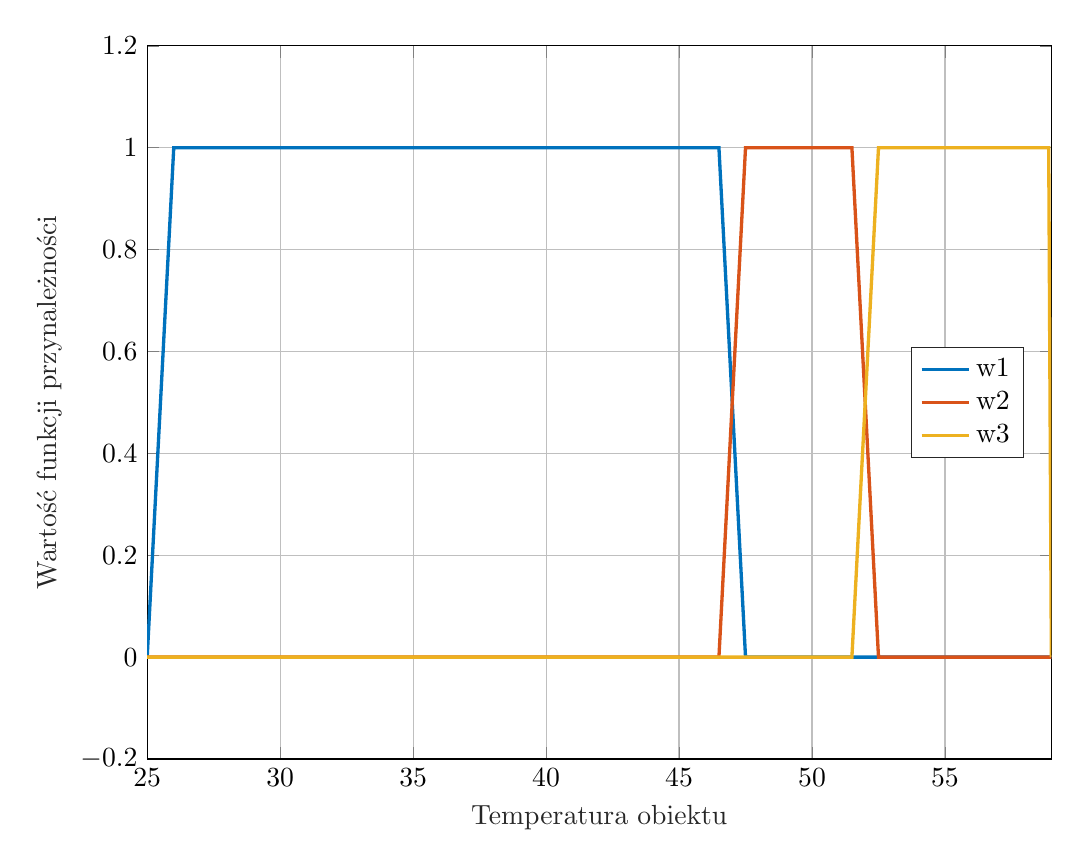
\begin{tikzpicture}

\begin{axis}[%
width=4.521in,
height=3.566in,
at={(0.758in,0.481in)},
scale only axis,
xmin=25,
xmax=59,
xlabel style={font=\color{white!15!black}},
xlabel={Temperatura obiektu},
ymin=-0.2,
ymax=1.2,
ylabel style={font=\color{white!15!black}},
ylabel={Wartość funkcji przynależności},
axis background/.style={fill=white},
xmajorgrids,
ymajorgrids,
legend style={at={(0.97,0.5)}, anchor=east, legend cell align=left, align=left, draw=white!15!black}
]
\addplot [color=mycolor1, line width=1.2pt]
  table[row sep=crcr]{%
25	-0.00100000000000122\\
25.1	0.0990000000000002\\
25.2	0.198999999999998\\
25.3	0.298999999999999\\
25.4	0.398999999999997\\
25.5	0.498999999999999\\
25.6	0.599\\
25.7	0.698999999999998\\
25.8	0.798999999999999\\
25.9	0.898999999999997\\
26	1\\
26.1	1\\
26.2	1\\
26.3	1\\
26.4	1\\
26.5	1\\
26.6	1\\
26.7	1\\
26.8	1\\
26.9	1\\
27	1\\
27.1	1\\
27.2	1\\
27.3	1\\
27.4	1\\
27.5	1\\
27.6	1\\
27.7	1\\
27.8	1\\
27.9	1\\
28	1\\
28.1	1\\
28.2	1\\
28.3	1\\
28.4	1\\
28.5	1\\
28.6	1\\
28.7	1\\
28.8	1\\
28.9	1\\
29	1\\
29.1	1\\
29.2	1\\
29.3	1\\
29.4	1\\
29.5	1\\
29.6	1\\
29.7	1\\
29.8	1\\
29.9	1\\
30	1\\
30.1	1\\
30.2	1\\
30.3	1\\
30.4	1\\
30.5	1\\
30.6	1\\
30.7	1\\
30.8	1\\
30.9	1\\
31	1\\
31.1	1\\
31.2	1\\
31.3	1\\
31.4	1\\
31.5	1\\
31.6	1\\
31.7	1\\
31.8	1\\
31.9	1\\
32	1\\
32.1	1\\
32.2	1\\
32.3	1\\
32.4	1\\
32.5	1\\
32.6	1\\
32.7	1\\
32.8	1\\
32.9	1\\
33	1\\
33.1	1\\
33.2	1\\
33.3	1\\
33.4	1\\
33.5	1\\
33.6	1\\
33.7	1\\
33.8	1\\
33.9	1\\
34	1\\
34.1	1\\
34.2	1\\
34.3	1\\
34.4	1\\
34.5	1\\
34.6	1\\
34.7	1\\
34.8	1\\
34.9	1\\
35	1\\
35.1	1\\
35.2	1\\
35.3	1\\
35.4	1\\
35.5	1\\
35.6	1\\
35.7	1\\
35.8	1\\
35.9	1\\
36	1\\
36.1	1\\
36.2	1\\
36.3	1\\
36.4	1\\
36.5	1\\
36.6	1\\
36.7	1\\
36.8	1\\
36.9	1\\
37	1\\
37.1	1\\
37.2	1\\
37.3	1\\
37.4	1\\
37.5	1\\
37.6	1\\
37.7	1\\
37.8	1\\
37.9	1\\
38	1\\
38.1	1\\
38.2	1\\
38.3	1\\
38.4	1\\
38.5	1\\
38.6	1\\
38.7	1\\
38.8	1\\
38.9	1\\
39	1\\
39.1	1\\
39.2	1\\
39.3	1\\
39.4	1\\
39.5	1\\
39.6	1\\
39.7	1\\
39.8	1\\
39.9	1\\
40	1\\
40.1	1\\
40.2	1\\
40.3	1\\
40.4	1\\
40.5	1\\
40.6	1\\
40.7	1\\
40.8	1\\
40.9	1\\
41	1\\
41.1	1\\
41.2	1\\
41.3	1\\
41.4	1\\
41.5	1\\
41.6	1\\
41.7	1\\
41.8	1\\
41.9	1\\
42	1\\
42.1	1\\
42.2	1\\
42.3	1\\
42.4	1\\
42.5	1\\
42.6	1\\
42.7	1\\
42.8	1\\
42.9	1\\
43	1\\
43.1	1\\
43.2	1\\
43.3	1\\
43.4	1\\
43.5	1\\
43.6	1\\
43.7	1\\
43.8	1\\
43.9	1\\
44	1\\
44.1	1\\
44.2	1\\
44.3	1\\
44.4	1\\
44.5	1\\
44.6	1\\
44.7	1\\
44.8	1\\
44.9	1\\
45	1\\
45.1	1\\
45.2	1\\
45.3	1\\
45.4	1\\
45.5	1\\
45.6	1\\
45.7	1\\
45.8	1\\
45.9	1\\
46	1\\
46.1	1\\
46.2	1\\
46.3	1\\
46.4	1\\
46.5	1\\
46.6	0.899999999999999\\
46.7	0.799999999999997\\
46.8	0.700000000000003\\
46.9	0.600000000000001\\
47	0.5\\
47.1	0.399999999999999\\
47.2	0.299999999999997\\
47.3	0.200000000000003\\
47.4	0.100000000000001\\
47.5	0\\
47.6	0\\
47.7	0\\
47.8	0\\
47.9	0\\
48	0\\
48.1	0\\
48.2	0\\
48.3	0\\
48.4	0\\
48.5	0\\
48.6	0\\
48.7	0\\
48.8	0\\
48.9	0\\
49	0\\
49.1	0\\
49.2	0\\
49.3	0\\
49.4	0\\
49.5	0\\
49.6	0\\
49.7	0\\
49.8	0\\
49.9	0\\
50	0\\
50.1	0\\
50.2	0\\
50.3	0\\
50.4	0\\
50.5	0\\
50.6	0\\
50.7	0\\
50.8	0\\
50.9	0\\
51	0\\
51.1	0\\
51.2	0\\
51.3	0\\
51.4	0\\
51.5	0\\
51.6	0\\
51.7	0\\
51.8	0\\
51.9	0\\
52	0\\
52.1	0\\
52.2	0\\
52.3	0\\
52.4	0\\
52.5	0\\
52.6	0\\
52.7	0\\
52.8	0\\
52.9	0\\
53	0\\
53.1	0\\
53.2	0\\
53.3	0\\
53.4	0\\
53.5	0\\
53.6	0\\
53.7	0\\
53.8	0\\
53.9	0\\
54	0\\
54.1	0\\
54.2	0\\
54.3	0\\
54.4	0\\
54.5	0\\
54.6	0\\
54.7	0\\
54.8	0\\
54.9	0\\
55	0\\
55.1	0\\
55.2	0\\
55.3	0\\
55.4	0\\
55.5	0\\
55.6	0\\
55.7	0\\
55.8	0\\
55.9	0\\
56	0\\
56.1	0\\
56.2	0\\
56.3	0\\
56.4	0\\
56.5	0\\
56.6	0\\
56.7	0\\
56.8	0\\
56.9	0\\
57	0\\
57.1	0\\
57.2	0\\
57.3	0\\
57.4	0\\
57.5	0\\
57.6	0\\
57.7	0\\
57.8	0\\
57.9	0\\
58	0\\
58.1	0\\
58.2	0\\
58.3	0\\
58.4	0\\
58.5	0\\
58.6	0\\
58.7	0\\
58.8	0\\
58.9	0\\
59	0\\
};
\addlegendentry{w1}

\addplot [color=mycolor2, line width=1.2pt]
  table[row sep=crcr]{%
25	0\\
25.1	0\\
25.2	0\\
25.3	0\\
25.4	0\\
25.5	0\\
25.6	0\\
25.7	0\\
25.8	0\\
25.9	0\\
26	0\\
26.1	0\\
26.2	0\\
26.3	0\\
26.4	0\\
26.5	0\\
26.6	0\\
26.7	0\\
26.8	0\\
26.9	0\\
27	0\\
27.1	0\\
27.2	0\\
27.3	0\\
27.4	0\\
27.5	0\\
27.6	0\\
27.7	0\\
27.8	0\\
27.9	0\\
28	0\\
28.1	0\\
28.2	0\\
28.3	0\\
28.4	0\\
28.5	0\\
28.6	0\\
28.7	0\\
28.8	0\\
28.9	0\\
29	0\\
29.1	0\\
29.2	0\\
29.3	0\\
29.4	0\\
29.5	0\\
29.6	0\\
29.7	0\\
29.8	0\\
29.9	0\\
30	0\\
30.1	0\\
30.2	0\\
30.3	0\\
30.4	0\\
30.5	0\\
30.6	0\\
30.7	0\\
30.8	0\\
30.9	0\\
31	0\\
31.1	0\\
31.2	0\\
31.3	0\\
31.4	0\\
31.5	0\\
31.6	0\\
31.7	0\\
31.8	0\\
31.9	0\\
32	0\\
32.1	0\\
32.2	0\\
32.3	0\\
32.4	0\\
32.5	0\\
32.6	0\\
32.7	0\\
32.8	0\\
32.9	0\\
33	0\\
33.1	0\\
33.2	0\\
33.3	0\\
33.4	0\\
33.5	0\\
33.6	0\\
33.7	0\\
33.8	0\\
33.9	0\\
34	0\\
34.1	0\\
34.2	0\\
34.3	0\\
34.4	0\\
34.5	0\\
34.6	0\\
34.7	0\\
34.8	0\\
34.9	0\\
35	0\\
35.1	0\\
35.2	0\\
35.3	0\\
35.4	0\\
35.5	0\\
35.6	0\\
35.7	0\\
35.8	0\\
35.9	0\\
36	0\\
36.1	0\\
36.2	0\\
36.3	0\\
36.4	0\\
36.5	0\\
36.6	0\\
36.7	0\\
36.8	0\\
36.9	0\\
37	0\\
37.1	0\\
37.2	0\\
37.3	0\\
37.4	0\\
37.5	0\\
37.6	0\\
37.7	0\\
37.8	0\\
37.9	0\\
38	0\\
38.1	0\\
38.2	0\\
38.3	0\\
38.4	0\\
38.5	0\\
38.6	0\\
38.7	0\\
38.8	0\\
38.9	0\\
39	0\\
39.1	0\\
39.2	0\\
39.3	0\\
39.4	0\\
39.5	0\\
39.6	0\\
39.7	0\\
39.8	0\\
39.9	0\\
40	0\\
40.1	0\\
40.2	0\\
40.3	0\\
40.4	0\\
40.5	0\\
40.6	0\\
40.7	0\\
40.8	0\\
40.9	0\\
41	0\\
41.1	0\\
41.2	0\\
41.3	0\\
41.4	0\\
41.5	0\\
41.6	0\\
41.7	0\\
41.8	0\\
41.9	0\\
42	0\\
42.1	0\\
42.2	0\\
42.3	0\\
42.4	0\\
42.5	0\\
42.6	0\\
42.7	0\\
42.8	0\\
42.9	0\\
43	0\\
43.1	0\\
43.2	0\\
43.3	0\\
43.4	0\\
43.5	0\\
43.6	0\\
43.7	0\\
43.8	0\\
43.9	0\\
44	0\\
44.1	0\\
44.2	0\\
44.3	0\\
44.4	0\\
44.5	0\\
44.6	0\\
44.7	0\\
44.8	0\\
44.9	0\\
45	0\\
45.1	0\\
45.2	0\\
45.3	0\\
45.4	0\\
45.5	0\\
45.6	0\\
45.7	0\\
45.8	0\\
45.9	0\\
46	0\\
46.1	0\\
46.2	0\\
46.3	0\\
46.4	0\\
46.5	0\\
46.6	0.100000000000001\\
46.7	0.200000000000003\\
46.8	0.299999999999997\\
46.9	0.399999999999999\\
47	0.5\\
47.1	0.600000000000001\\
47.2	0.700000000000003\\
47.3	0.799999999999997\\
47.4	0.899999999999999\\
47.5	1\\
47.6	1\\
47.7	1\\
47.8	1\\
47.9	1\\
48	1\\
48.1	1\\
48.2	1\\
48.3	1\\
48.4	1\\
48.5	1\\
48.6	1\\
48.7	1\\
48.8	1\\
48.9	1\\
49	1\\
49.1	1\\
49.2	1\\
49.3	1\\
49.4	1\\
49.5	1\\
49.6	1\\
49.7	1\\
49.8	1\\
49.9	1\\
50	1\\
50.1	1\\
50.2	1\\
50.3	1\\
50.4	1\\
50.5	1\\
50.6	1\\
50.7	1\\
50.8	1\\
50.9	1\\
51	1\\
51.1	1\\
51.2	1\\
51.3	1\\
51.4	1\\
51.5	1\\
51.6	0.899999999999999\\
51.7	0.799999999999997\\
51.8	0.700000000000003\\
51.9	0.600000000000001\\
52	0.5\\
52.1	0.399999999999999\\
52.2	0.299999999999997\\
52.3	0.200000000000003\\
52.4	0.100000000000001\\
52.5	0\\
52.6	0\\
52.7	0\\
52.8	0\\
52.9	0\\
53	0\\
53.1	0\\
53.2	0\\
53.3	0\\
53.4	0\\
53.5	0\\
53.6	0\\
53.7	0\\
53.8	0\\
53.9	0\\
54	0\\
54.1	0\\
54.2	0\\
54.3	0\\
54.4	0\\
54.5	0\\
54.6	0\\
54.7	0\\
54.8	0\\
54.9	0\\
55	0\\
55.1	0\\
55.2	0\\
55.3	0\\
55.4	0\\
55.5	0\\
55.6	0\\
55.7	0\\
55.8	0\\
55.9	0\\
56	0\\
56.1	0\\
56.2	0\\
56.3	0\\
56.4	0\\
56.5	0\\
56.6	0\\
56.7	0\\
56.8	0\\
56.9	0\\
57	0\\
57.1	0\\
57.2	0\\
57.3	0\\
57.4	0\\
57.5	0\\
57.6	0\\
57.7	0\\
57.8	0\\
57.9	0\\
58	0\\
58.1	0\\
58.2	0\\
58.3	0\\
58.4	0\\
58.5	0\\
58.6	0\\
58.7	0\\
58.8	0\\
58.9	0\\
59	0\\
};
\addlegendentry{w2}

\addplot [color=mycolor3, line width=1.2pt]
  table[row sep=crcr]{%
25	0\\
25.1	0\\
25.2	0\\
25.3	0\\
25.4	0\\
25.5	0\\
25.6	0\\
25.7	0\\
25.8	0\\
25.9	0\\
26	0\\
26.1	0\\
26.2	0\\
26.3	0\\
26.4	0\\
26.5	0\\
26.6	0\\
26.7	0\\
26.8	0\\
26.9	0\\
27	0\\
27.1	0\\
27.2	0\\
27.3	0\\
27.4	0\\
27.5	0\\
27.6	0\\
27.7	0\\
27.8	0\\
27.9	0\\
28	0\\
28.1	0\\
28.2	0\\
28.3	0\\
28.4	0\\
28.5	0\\
28.6	0\\
28.7	0\\
28.8	0\\
28.9	0\\
29	0\\
29.1	0\\
29.2	0\\
29.3	0\\
29.4	0\\
29.5	0\\
29.6	0\\
29.7	0\\
29.8	0\\
29.9	0\\
30	0\\
30.1	0\\
30.2	0\\
30.3	0\\
30.4	0\\
30.5	0\\
30.6	0\\
30.7	0\\
30.8	0\\
30.9	0\\
31	0\\
31.1	0\\
31.2	0\\
31.3	0\\
31.4	0\\
31.5	0\\
31.6	0\\
31.7	0\\
31.8	0\\
31.9	0\\
32	0\\
32.1	0\\
32.2	0\\
32.3	0\\
32.4	0\\
32.5	0\\
32.6	0\\
32.7	0\\
32.8	0\\
32.9	0\\
33	0\\
33.1	0\\
33.2	0\\
33.3	0\\
33.4	0\\
33.5	0\\
33.6	0\\
33.7	0\\
33.8	0\\
33.9	0\\
34	0\\
34.1	0\\
34.2	0\\
34.3	0\\
34.4	0\\
34.5	0\\
34.6	0\\
34.7	0\\
34.8	0\\
34.9	0\\
35	0\\
35.1	0\\
35.2	0\\
35.3	0\\
35.4	0\\
35.5	0\\
35.6	0\\
35.7	0\\
35.8	0\\
35.9	0\\
36	0\\
36.1	0\\
36.2	0\\
36.3	0\\
36.4	0\\
36.5	0\\
36.6	0\\
36.7	0\\
36.8	0\\
36.9	0\\
37	0\\
37.1	0\\
37.2	0\\
37.3	0\\
37.4	0\\
37.5	0\\
37.6	0\\
37.7	0\\
37.8	0\\
37.9	0\\
38	0\\
38.1	0\\
38.2	0\\
38.3	0\\
38.4	0\\
38.5	0\\
38.6	0\\
38.7	0\\
38.8	0\\
38.9	0\\
39	0\\
39.1	0\\
39.2	0\\
39.3	0\\
39.4	0\\
39.5	0\\
39.6	0\\
39.7	0\\
39.8	0\\
39.9	0\\
40	0\\
40.1	0\\
40.2	0\\
40.3	0\\
40.4	0\\
40.5	0\\
40.6	0\\
40.7	0\\
40.8	0\\
40.9	0\\
41	0\\
41.1	0\\
41.2	0\\
41.3	0\\
41.4	0\\
41.5	0\\
41.6	0\\
41.7	0\\
41.8	0\\
41.9	0\\
42	0\\
42.1	0\\
42.2	0\\
42.3	0\\
42.4	0\\
42.5	0\\
42.6	0\\
42.7	0\\
42.8	0\\
42.9	0\\
43	0\\
43.1	0\\
43.2	0\\
43.3	0\\
43.4	0\\
43.5	0\\
43.6	0\\
43.7	0\\
43.8	0\\
43.9	0\\
44	0\\
44.1	0\\
44.2	0\\
44.3	0\\
44.4	0\\
44.5	0\\
44.6	0\\
44.7	0\\
44.8	0\\
44.9	0\\
45	0\\
45.1	0\\
45.2	0\\
45.3	0\\
45.4	0\\
45.5	0\\
45.6	0\\
45.7	0\\
45.8	0\\
45.9	0\\
46	0\\
46.1	0\\
46.2	0\\
46.3	0\\
46.4	0\\
46.5	0\\
46.6	0\\
46.7	0\\
46.8	0\\
46.9	0\\
47	0\\
47.1	0\\
47.2	0\\
47.3	0\\
47.4	0\\
47.5	0\\
47.6	0\\
47.7	0\\
47.8	0\\
47.9	0\\
48	0\\
48.1	0\\
48.2	0\\
48.3	0\\
48.4	0\\
48.5	0\\
48.6	0\\
48.7	0\\
48.8	0\\
48.9	0\\
49	0\\
49.1	0\\
49.2	0\\
49.3	0\\
49.4	0\\
49.5	0\\
49.6	0\\
49.7	0\\
49.8	0\\
49.9	0\\
50	0\\
50.1	0\\
50.2	0\\
50.3	0\\
50.4	0\\
50.5	0\\
50.6	0\\
50.7	0\\
50.8	0\\
50.9	0\\
51	0\\
51.1	0\\
51.2	0\\
51.3	0\\
51.4	0\\
51.5	0\\
51.6	0.100000000000001\\
51.7	0.200000000000003\\
51.8	0.299999999999997\\
51.9	0.399999999999999\\
52	0.5\\
52.1	0.600000000000001\\
52.2	0.700000000000003\\
52.3	0.799999999999997\\
52.4	0.899999999999999\\
52.5	1\\
52.6	1\\
52.7	1\\
52.8	1\\
52.9	1\\
53	1\\
53.1	1\\
53.2	1\\
53.3	1\\
53.4	1\\
53.5	1\\
53.6	1\\
53.7	1\\
53.8	1\\
53.9	1\\
54	1\\
54.1	1\\
54.2	1\\
54.3	1\\
54.4	1\\
54.5	1\\
54.6	1\\
54.7	1\\
54.8	1\\
54.9	1\\
55	1\\
55.1	1\\
55.2	1\\
55.3	1\\
55.4	1\\
55.5	1\\
55.6	1\\
55.7	1\\
55.8	1\\
55.9	1\\
56	1\\
56.1	1\\
56.2	1\\
56.3	1\\
56.4	1\\
56.5	1\\
56.6	1\\
56.7	1\\
56.8	1\\
56.9	1\\
57	1\\
57.1	1\\
57.2	1\\
57.3	1\\
57.4	1\\
57.5	1\\
57.6	1\\
57.7	1\\
57.8	1\\
57.9	1\\
58	1\\
58.1	1\\
58.2	1\\
58.3	1\\
58.4	1\\
58.5	1\\
58.6	1\\
58.7	1\\
58.8	1\\
58.9	1\\
59	0\\
};
\addlegendentry{w3}

\end{axis}
\end{tikzpicture}%
    \caption{Funkcje rozmycia}
    \label{lab:zad4:fuzzyFunction:figure}
 \end{figure}

\newpage

\subsection{Implementacja rozmytego algorytmu PID}
\label{lab:zad4:implPID}


\newpage

\subsection{Dobór parametrów lokalnych regulatorów PID}
\label{lab:zad4:paramPID}

\begin{figure}[H] 
    \centering
    % This file was created by matlab2tikz.
%
\definecolor{mycolor1}{rgb}{0.00000,0.44700,0.74100}%
\definecolor{mycolor2}{rgb}{0.85000,0.32500,0.09800}%
%
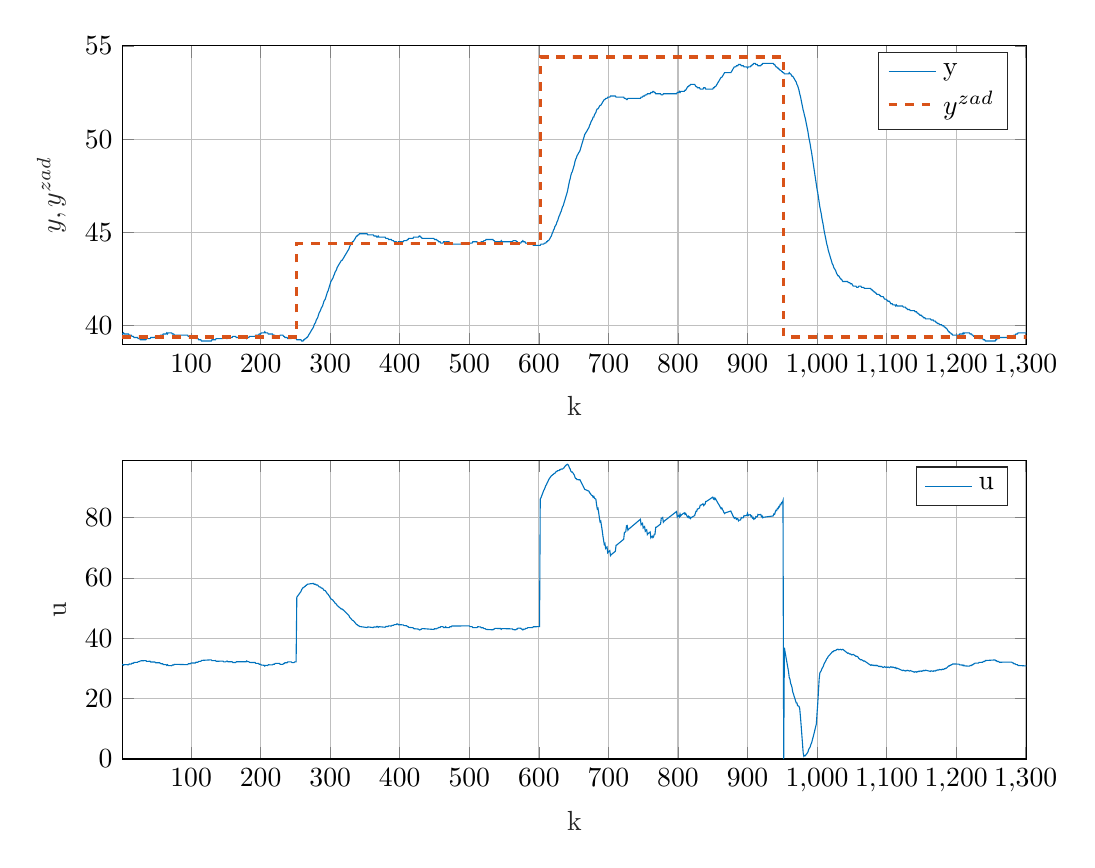
\begin{tikzpicture}

\begin{axis}[%
width=4.521in,
height=1.493in,
at={(0.758in,2.554in)},
scale only axis,
xmin=1,
xmax=1301,
xlabel style={font=\color{white!15!black}},
xlabel={k},
ymin=39,
ymax=55,
ylabel style={font=\color{white!15!black}},
ylabel={$\text{y, y}^{\text{zad}}$},
axis background/.style={fill=white},
xmajorgrids,
ymajorgrids,
legend style={legend cell align=left, align=left, draw=white!15!black}
]
\addplot [color=mycolor1]
  table[row sep=crcr]{%
1	39.56\\
2	39.56\\
3	39.62\\
4	39.56\\
5	39.56\\
6	39.56\\
7	39.56\\
8	39.56\\
9	39.56\\
10	39.56\\
11	39.5\\
12	39.5\\
13	39.5\\
14	39.5\\
15	39.43\\
16	39.43\\
17	39.43\\
18	39.37\\
19	39.37\\
20	39.37\\
21	39.37\\
22	39.37\\
23	39.37\\
24	39.31\\
25	39.31\\
26	39.31\\
27	39.25\\
28	39.25\\
29	39.25\\
30	39.25\\
31	39.25\\
32	39.25\\
33	39.25\\
34	39.25\\
35	39.25\\
36	39.31\\
37	39.31\\
38	39.31\\
39	39.31\\
40	39.31\\
41	39.31\\
42	39.37\\
43	39.37\\
44	39.37\\
45	39.37\\
46	39.37\\
47	39.37\\
48	39.37\\
49	39.43\\
50	39.43\\
51	39.43\\
52	39.43\\
53	39.43\\
54	39.43\\
55	39.43\\
56	39.5\\
57	39.5\\
58	39.5\\
59	39.5\\
60	39.56\\
61	39.56\\
62	39.56\\
63	39.56\\
64	39.56\\
65	39.62\\
66	39.56\\
67	39.62\\
68	39.62\\
69	39.62\\
70	39.62\\
71	39.62\\
72	39.62\\
73	39.56\\
74	39.56\\
75	39.56\\
76	39.5\\
77	39.5\\
78	39.5\\
79	39.5\\
80	39.5\\
81	39.5\\
82	39.5\\
83	39.5\\
84	39.5\\
85	39.5\\
86	39.5\\
87	39.5\\
88	39.5\\
89	39.5\\
90	39.5\\
91	39.5\\
92	39.5\\
93	39.5\\
94	39.5\\
95	39.5\\
96	39.43\\
97	39.43\\
98	39.43\\
99	39.43\\
100	39.37\\
101	39.37\\
102	39.37\\
103	39.37\\
104	39.37\\
105	39.37\\
106	39.37\\
107	39.31\\
108	39.31\\
109	39.31\\
110	39.31\\
111	39.25\\
112	39.25\\
113	39.25\\
114	39.25\\
115	39.18\\
116	39.18\\
117	39.18\\
118	39.18\\
119	39.18\\
120	39.18\\
121	39.18\\
122	39.18\\
123	39.18\\
124	39.18\\
125	39.18\\
126	39.18\\
127	39.18\\
128	39.18\\
129	39.18\\
130	39.25\\
131	39.25\\
132	39.25\\
133	39.25\\
134	39.25\\
135	39.25\\
136	39.31\\
137	39.31\\
138	39.31\\
139	39.31\\
140	39.31\\
141	39.31\\
142	39.31\\
143	39.31\\
144	39.31\\
145	39.31\\
146	39.31\\
147	39.37\\
148	39.37\\
149	39.37\\
150	39.37\\
151	39.31\\
152	39.31\\
153	39.37\\
154	39.37\\
155	39.37\\
156	39.37\\
157	39.37\\
158	39.37\\
159	39.37\\
160	39.43\\
161	39.43\\
162	39.43\\
163	39.43\\
164	39.43\\
165	39.37\\
166	39.37\\
167	39.37\\
168	39.37\\
169	39.37\\
170	39.37\\
171	39.37\\
172	39.37\\
173	39.37\\
174	39.37\\
175	39.37\\
176	39.37\\
177	39.37\\
178	39.37\\
179	39.37\\
180	39.31\\
181	39.37\\
182	39.37\\
183	39.37\\
184	39.43\\
185	39.43\\
186	39.43\\
187	39.43\\
188	39.43\\
189	39.43\\
190	39.43\\
191	39.43\\
192	39.43\\
193	39.5\\
194	39.5\\
195	39.5\\
196	39.5\\
197	39.5\\
198	39.56\\
199	39.56\\
200	39.56\\
201	39.62\\
202	39.62\\
203	39.62\\
204	39.62\\
205	39.62\\
206	39.68\\
207	39.62\\
208	39.62\\
209	39.62\\
210	39.62\\
211	39.56\\
212	39.56\\
213	39.56\\
214	39.56\\
215	39.56\\
216	39.56\\
217	39.56\\
218	39.5\\
219	39.5\\
220	39.5\\
221	39.43\\
222	39.43\\
223	39.43\\
224	39.43\\
225	39.43\\
226	39.43\\
227	39.43\\
228	39.5\\
229	39.5\\
230	39.5\\
231	39.5\\
232	39.5\\
233	39.43\\
234	39.43\\
235	39.37\\
236	39.37\\
237	39.37\\
238	39.37\\
239	39.31\\
240	39.31\\
241	39.31\\
242	39.31\\
243	39.31\\
244	39.31\\
245	39.37\\
246	39.37\\
247	39.37\\
248	39.37\\
249	39.31\\
250	39.31\\
251	39.31\\
252	39.25\\
253	39.25\\
254	39.25\\
255	39.25\\
256	39.25\\
257	39.25\\
258	39.25\\
259	39.18\\
260	39.18\\
261	39.18\\
262	39.25\\
263	39.25\\
264	39.31\\
265	39.31\\
266	39.37\\
267	39.37\\
268	39.43\\
269	39.5\\
270	39.56\\
271	39.62\\
272	39.68\\
273	39.75\\
274	39.81\\
275	39.87\\
276	39.93\\
277	40.06\\
278	40.12\\
279	40.18\\
280	40.31\\
281	40.37\\
282	40.43\\
283	40.56\\
284	40.68\\
285	40.75\\
286	40.81\\
287	40.93\\
288	41\\
289	41.06\\
290	41.18\\
291	41.31\\
292	41.37\\
293	41.43\\
294	41.56\\
295	41.68\\
296	41.81\\
297	41.87\\
298	42\\
299	42.12\\
300	42.25\\
301	42.37\\
302	42.43\\
303	42.5\\
304	42.56\\
305	42.68\\
306	42.75\\
307	42.87\\
308	42.93\\
309	43\\
310	43.12\\
311	43.18\\
312	43.25\\
313	43.31\\
314	43.37\\
315	43.43\\
316	43.5\\
317	43.5\\
318	43.56\\
319	43.62\\
320	43.68\\
321	43.75\\
322	43.81\\
323	43.87\\
324	43.93\\
325	44\\
326	44.06\\
327	44.12\\
328	44.25\\
329	44.31\\
330	44.37\\
331	44.43\\
332	44.5\\
333	44.5\\
334	44.56\\
335	44.62\\
336	44.68\\
337	44.75\\
338	44.81\\
339	44.81\\
340	44.87\\
341	44.87\\
342	44.93\\
343	44.93\\
344	44.93\\
345	44.93\\
346	44.93\\
347	44.93\\
348	44.93\\
349	44.93\\
350	44.93\\
351	44.93\\
352	44.93\\
353	44.93\\
354	44.87\\
355	44.87\\
356	44.87\\
357	44.87\\
358	44.87\\
359	44.87\\
360	44.87\\
361	44.87\\
362	44.87\\
363	44.81\\
364	44.81\\
365	44.81\\
366	44.81\\
367	44.75\\
368	44.75\\
369	44.81\\
370	44.75\\
371	44.75\\
372	44.75\\
373	44.75\\
374	44.75\\
375	44.75\\
376	44.75\\
377	44.75\\
378	44.75\\
379	44.75\\
380	44.68\\
381	44.68\\
382	44.68\\
383	44.68\\
384	44.62\\
385	44.62\\
386	44.62\\
387	44.62\\
388	44.62\\
389	44.56\\
390	44.56\\
391	44.56\\
392	44.5\\
393	44.5\\
394	44.5\\
395	44.5\\
396	44.43\\
397	44.43\\
398	44.5\\
399	44.5\\
400	44.5\\
401	44.5\\
402	44.5\\
403	44.5\\
404	44.5\\
405	44.5\\
406	44.56\\
407	44.56\\
408	44.56\\
409	44.56\\
410	44.56\\
411	44.62\\
412	44.62\\
413	44.68\\
414	44.68\\
415	44.68\\
416	44.68\\
417	44.68\\
418	44.68\\
419	44.68\\
420	44.75\\
421	44.75\\
422	44.75\\
423	44.75\\
424	44.75\\
425	44.75\\
426	44.75\\
427	44.75\\
428	44.81\\
429	44.81\\
430	44.75\\
431	44.75\\
432	44.68\\
433	44.68\\
434	44.68\\
435	44.68\\
436	44.68\\
437	44.68\\
438	44.68\\
439	44.68\\
440	44.68\\
441	44.68\\
442	44.68\\
443	44.68\\
444	44.68\\
445	44.68\\
446	44.68\\
447	44.68\\
448	44.68\\
449	44.68\\
450	44.62\\
451	44.62\\
452	44.62\\
453	44.62\\
454	44.56\\
455	44.56\\
456	44.5\\
457	44.5\\
458	44.5\\
459	44.43\\
460	44.43\\
461	44.43\\
462	44.43\\
463	44.5\\
464	44.5\\
465	44.5\\
466	44.43\\
467	44.5\\
468	44.5\\
469	44.5\\
470	44.5\\
471	44.5\\
472	44.43\\
473	44.43\\
474	44.43\\
475	44.37\\
476	44.37\\
477	44.37\\
478	44.37\\
479	44.37\\
480	44.37\\
481	44.37\\
482	44.37\\
483	44.37\\
484	44.37\\
485	44.37\\
486	44.37\\
487	44.37\\
488	44.37\\
489	44.37\\
490	44.37\\
491	44.37\\
492	44.37\\
493	44.37\\
494	44.37\\
495	44.37\\
496	44.37\\
497	44.37\\
498	44.37\\
499	44.37\\
500	44.37\\
501	44.43\\
502	44.43\\
503	44.43\\
504	44.43\\
505	44.5\\
506	44.5\\
507	44.5\\
508	44.5\\
509	44.5\\
510	44.5\\
511	44.5\\
512	44.43\\
513	44.43\\
514	44.43\\
515	44.43\\
516	44.43\\
517	44.5\\
518	44.5\\
519	44.5\\
520	44.5\\
521	44.56\\
522	44.56\\
523	44.56\\
524	44.62\\
525	44.62\\
526	44.62\\
527	44.62\\
528	44.62\\
529	44.62\\
530	44.62\\
531	44.62\\
532	44.62\\
533	44.62\\
534	44.62\\
535	44.56\\
536	44.56\\
537	44.5\\
538	44.5\\
539	44.5\\
540	44.5\\
541	44.5\\
542	44.5\\
543	44.5\\
544	44.5\\
545	44.5\\
546	44.56\\
547	44.5\\
548	44.5\\
549	44.5\\
550	44.5\\
551	44.5\\
552	44.5\\
553	44.5\\
554	44.5\\
555	44.5\\
556	44.5\\
557	44.5\\
558	44.5\\
559	44.5\\
560	44.5\\
561	44.5\\
562	44.5\\
563	44.56\\
564	44.56\\
565	44.56\\
566	44.56\\
567	44.56\\
568	44.5\\
569	44.5\\
570	44.43\\
571	44.43\\
572	44.43\\
573	44.43\\
574	44.43\\
575	44.5\\
576	44.5\\
577	44.56\\
578	44.5\\
579	44.5\\
580	44.5\\
581	44.43\\
582	44.43\\
583	44.43\\
584	44.37\\
585	44.37\\
586	44.37\\
587	44.37\\
588	44.37\\
589	44.37\\
590	44.37\\
591	44.37\\
592	44.31\\
593	44.31\\
594	44.31\\
595	44.31\\
596	44.31\\
597	44.31\\
598	44.31\\
599	44.31\\
600	44.31\\
601	44.31\\
602	44.31\\
603	44.37\\
604	44.37\\
605	44.37\\
606	44.37\\
607	44.37\\
608	44.43\\
609	44.43\\
610	44.43\\
611	44.5\\
612	44.5\\
613	44.56\\
614	44.56\\
615	44.62\\
616	44.68\\
617	44.75\\
618	44.81\\
619	44.93\\
620	45\\
621	45.12\\
622	45.18\\
623	45.31\\
624	45.37\\
625	45.43\\
626	45.56\\
627	45.62\\
628	45.75\\
629	45.87\\
630	45.93\\
631	46.06\\
632	46.12\\
633	46.25\\
634	46.37\\
635	46.43\\
636	46.56\\
637	46.68\\
638	46.81\\
639	46.93\\
640	47.06\\
641	47.18\\
642	47.37\\
643	47.56\\
644	47.75\\
645	47.87\\
646	48.06\\
647	48.18\\
648	48.25\\
649	48.37\\
650	48.5\\
651	48.62\\
652	48.81\\
653	48.93\\
654	49\\
655	49.12\\
656	49.18\\
657	49.25\\
658	49.31\\
659	49.37\\
660	49.5\\
661	49.62\\
662	49.75\\
663	49.87\\
664	50\\
665	50.12\\
666	50.25\\
667	50.31\\
668	50.37\\
669	50.43\\
670	50.5\\
671	50.56\\
672	50.62\\
673	50.75\\
674	50.81\\
675	50.93\\
676	51\\
677	51.06\\
678	51.18\\
679	51.18\\
680	51.31\\
681	51.37\\
682	51.43\\
683	51.56\\
684	51.62\\
685	51.62\\
686	51.68\\
687	51.75\\
688	51.81\\
689	51.81\\
690	51.87\\
691	51.93\\
692	52\\
693	52.06\\
694	52.12\\
695	52.12\\
696	52.18\\
697	52.18\\
698	52.18\\
699	52.25\\
700	52.25\\
701	52.25\\
702	52.25\\
703	52.31\\
704	52.31\\
705	52.31\\
706	52.31\\
707	52.31\\
708	52.31\\
709	52.31\\
710	52.31\\
711	52.25\\
712	52.25\\
713	52.25\\
714	52.25\\
715	52.25\\
716	52.25\\
717	52.25\\
718	52.25\\
719	52.25\\
720	52.25\\
721	52.25\\
722	52.25\\
723	52.18\\
724	52.18\\
725	52.18\\
726	52.12\\
727	52.12\\
728	52.18\\
729	52.18\\
730	52.18\\
731	52.18\\
732	52.18\\
733	52.18\\
734	52.18\\
735	52.18\\
736	52.18\\
737	52.18\\
738	52.18\\
739	52.18\\
740	52.18\\
741	52.18\\
742	52.18\\
743	52.18\\
744	52.18\\
745	52.18\\
746	52.18\\
747	52.25\\
748	52.25\\
749	52.25\\
750	52.31\\
751	52.31\\
752	52.31\\
753	52.37\\
754	52.37\\
755	52.37\\
756	52.43\\
757	52.43\\
758	52.43\\
759	52.43\\
760	52.43\\
761	52.5\\
762	52.5\\
763	52.5\\
764	52.56\\
765	52.56\\
766	52.5\\
767	52.5\\
768	52.43\\
769	52.43\\
770	52.43\\
771	52.43\\
772	52.43\\
773	52.43\\
774	52.43\\
775	52.43\\
776	52.37\\
777	52.37\\
778	52.37\\
779	52.43\\
780	52.43\\
781	52.43\\
782	52.43\\
783	52.43\\
784	52.43\\
785	52.43\\
786	52.43\\
787	52.43\\
788	52.43\\
789	52.43\\
790	52.43\\
791	52.43\\
792	52.43\\
793	52.43\\
794	52.43\\
795	52.43\\
796	52.43\\
797	52.43\\
798	52.43\\
799	52.5\\
800	52.5\\
801	52.5\\
802	52.56\\
803	52.5\\
804	52.56\\
805	52.56\\
806	52.56\\
807	52.56\\
808	52.56\\
809	52.56\\
810	52.62\\
811	52.62\\
812	52.68\\
813	52.75\\
814	52.81\\
815	52.81\\
816	52.87\\
817	52.87\\
818	52.93\\
819	52.93\\
820	52.93\\
821	52.93\\
822	52.93\\
823	52.93\\
824	52.93\\
825	52.87\\
826	52.81\\
827	52.81\\
828	52.75\\
829	52.75\\
830	52.75\\
831	52.75\\
832	52.68\\
833	52.68\\
834	52.68\\
835	52.68\\
836	52.68\\
837	52.75\\
838	52.75\\
839	52.75\\
840	52.68\\
841	52.68\\
842	52.68\\
843	52.68\\
844	52.68\\
845	52.68\\
846	52.68\\
847	52.68\\
848	52.68\\
849	52.68\\
850	52.68\\
851	52.75\\
852	52.75\\
853	52.81\\
854	52.81\\
855	52.87\\
856	52.93\\
857	53\\
858	53.06\\
859	53.12\\
860	53.18\\
861	53.25\\
862	53.31\\
863	53.31\\
864	53.37\\
865	53.43\\
866	53.5\\
867	53.56\\
868	53.56\\
869	53.56\\
870	53.56\\
871	53.56\\
872	53.56\\
873	53.56\\
874	53.56\\
875	53.56\\
876	53.56\\
877	53.62\\
878	53.68\\
879	53.75\\
880	53.81\\
881	53.87\\
882	53.87\\
883	53.87\\
884	53.93\\
885	53.93\\
886	53.93\\
887	54\\
888	54\\
889	54\\
890	54\\
891	53.93\\
892	53.93\\
893	53.93\\
894	53.93\\
895	53.87\\
896	53.87\\
897	53.87\\
898	53.87\\
899	53.87\\
900	53.81\\
901	53.87\\
902	53.87\\
903	53.87\\
904	53.87\\
905	53.93\\
906	53.93\\
907	54\\
908	54\\
909	54.06\\
910	54.06\\
911	54.06\\
912	54\\
913	54\\
914	54\\
915	53.93\\
916	53.93\\
917	53.93\\
918	53.93\\
919	53.93\\
920	54\\
921	54\\
922	54.06\\
923	54.06\\
924	54.06\\
925	54.06\\
926	54.06\\
927	54.06\\
928	54.06\\
929	54.06\\
930	54.06\\
931	54.06\\
932	54.06\\
933	54.06\\
934	54.06\\
935	54.06\\
936	54.06\\
937	54.06\\
938	54\\
939	54\\
940	53.93\\
941	53.87\\
942	53.87\\
943	53.81\\
944	53.81\\
945	53.75\\
946	53.75\\
947	53.68\\
948	53.68\\
949	53.62\\
950	53.62\\
951	53.56\\
952	53.56\\
953	53.5\\
954	53.5\\
955	53.5\\
956	53.5\\
957	53.5\\
958	53.5\\
959	53.5\\
960	53.56\\
961	53.5\\
962	53.5\\
963	53.43\\
964	53.37\\
965	53.37\\
966	53.31\\
967	53.25\\
968	53.18\\
969	53.12\\
970	53.06\\
971	52.93\\
972	52.87\\
973	52.75\\
974	52.62\\
975	52.43\\
976	52.31\\
977	52.12\\
978	51.93\\
979	51.75\\
980	51.56\\
981	51.43\\
982	51.25\\
983	51.12\\
984	50.93\\
985	50.75\\
986	50.56\\
987	50.37\\
988	50.12\\
989	49.93\\
990	49.75\\
991	49.5\\
992	49.31\\
993	49.06\\
994	48.81\\
995	48.56\\
996	48.31\\
997	48.06\\
998	47.81\\
999	47.56\\
1000	47.31\\
1001	47.12\\
1002	46.87\\
1003	46.62\\
1004	46.37\\
1005	46.18\\
1006	46\\
1007	45.75\\
1008	45.56\\
1009	45.37\\
1010	45.12\\
1011	44.93\\
1012	44.75\\
1013	44.56\\
1014	44.37\\
1015	44.25\\
1016	44.06\\
1017	43.93\\
1018	43.81\\
1019	43.68\\
1020	43.56\\
1021	43.43\\
1022	43.31\\
1023	43.25\\
1024	43.12\\
1025	43.06\\
1026	43\\
1027	42.93\\
1028	42.81\\
1029	42.75\\
1030	42.68\\
1031	42.68\\
1032	42.62\\
1033	42.56\\
1034	42.5\\
1035	42.5\\
1036	42.43\\
1037	42.37\\
1038	42.37\\
1039	42.37\\
1040	42.37\\
1041	42.37\\
1042	42.37\\
1043	42.37\\
1044	42.37\\
1045	42.31\\
1046	42.31\\
1047	42.31\\
1048	42.25\\
1049	42.25\\
1050	42.25\\
1051	42.18\\
1052	42.12\\
1053	42.12\\
1054	42.12\\
1055	42.12\\
1056	42.12\\
1057	42.06\\
1058	42.06\\
1059	42.06\\
1060	42.12\\
1061	42.12\\
1062	42.12\\
1063	42.12\\
1064	42.06\\
1065	42.06\\
1066	42.06\\
1067	42.06\\
1068	42\\
1069	42\\
1070	42\\
1071	42\\
1072	42\\
1073	42\\
1074	42\\
1075	42\\
1076	42\\
1077	42\\
1078	41.93\\
1079	41.93\\
1080	41.87\\
1081	41.87\\
1082	41.81\\
1083	41.81\\
1084	41.75\\
1085	41.75\\
1086	41.68\\
1087	41.68\\
1088	41.68\\
1089	41.68\\
1090	41.62\\
1091	41.62\\
1092	41.56\\
1093	41.56\\
1094	41.56\\
1095	41.56\\
1096	41.5\\
1097	41.43\\
1098	41.43\\
1099	41.43\\
1100	41.37\\
1101	41.37\\
1102	41.31\\
1103	41.31\\
1104	41.31\\
1105	41.25\\
1106	41.18\\
1107	41.18\\
1108	41.18\\
1109	41.12\\
1110	41.12\\
1111	41.12\\
1112	41.12\\
1113	41.06\\
1114	41.12\\
1115	41.06\\
1116	41.06\\
1117	41.06\\
1118	41.06\\
1119	41.06\\
1120	41.06\\
1121	41.06\\
1122	41.06\\
1123	41.06\\
1124	41\\
1125	41\\
1126	41\\
1127	41\\
1128	40.93\\
1129	40.93\\
1130	40.87\\
1131	40.87\\
1132	40.87\\
1133	40.87\\
1134	40.81\\
1135	40.81\\
1136	40.81\\
1137	40.81\\
1138	40.81\\
1139	40.81\\
1140	40.81\\
1141	40.75\\
1142	40.75\\
1143	40.75\\
1144	40.68\\
1145	40.68\\
1146	40.62\\
1147	40.62\\
1148	40.56\\
1149	40.56\\
1150	40.56\\
1151	40.5\\
1152	40.5\\
1153	40.43\\
1154	40.43\\
1155	40.43\\
1156	40.37\\
1157	40.37\\
1158	40.37\\
1159	40.37\\
1160	40.37\\
1161	40.37\\
1162	40.37\\
1163	40.37\\
1164	40.31\\
1165	40.31\\
1166	40.31\\
1167	40.31\\
1168	40.25\\
1169	40.25\\
1170	40.25\\
1171	40.18\\
1172	40.18\\
1173	40.12\\
1174	40.12\\
1175	40.12\\
1176	40.06\\
1177	40.06\\
1178	40.06\\
1179	40.06\\
1180	40\\
1181	40\\
1182	40\\
1183	39.93\\
1184	39.93\\
1185	39.87\\
1186	39.87\\
1187	39.81\\
1188	39.75\\
1189	39.68\\
1190	39.68\\
1191	39.62\\
1192	39.62\\
1193	39.56\\
1194	39.56\\
1195	39.5\\
1196	39.5\\
1197	39.5\\
1198	39.5\\
1199	39.5\\
1200	39.5\\
1201	39.5\\
1202	39.5\\
1203	39.5\\
1204	39.5\\
1205	39.56\\
1206	39.56\\
1207	39.56\\
1208	39.56\\
1209	39.56\\
1210	39.62\\
1211	39.56\\
1212	39.62\\
1213	39.62\\
1214	39.62\\
1215	39.62\\
1216	39.62\\
1217	39.62\\
1218	39.62\\
1219	39.62\\
1220	39.56\\
1221	39.56\\
1222	39.56\\
1223	39.5\\
1224	39.5\\
1225	39.43\\
1226	39.43\\
1227	39.37\\
1228	39.37\\
1229	39.37\\
1230	39.37\\
1231	39.37\\
1232	39.37\\
1233	39.31\\
1234	39.31\\
1235	39.31\\
1236	39.31\\
1237	39.31\\
1238	39.31\\
1239	39.25\\
1240	39.25\\
1241	39.25\\
1242	39.18\\
1243	39.18\\
1244	39.18\\
1245	39.18\\
1246	39.18\\
1247	39.18\\
1248	39.18\\
1249	39.18\\
1250	39.18\\
1251	39.18\\
1252	39.18\\
1253	39.18\\
1254	39.18\\
1255	39.18\\
1256	39.18\\
1257	39.25\\
1258	39.25\\
1259	39.31\\
1260	39.31\\
1261	39.31\\
1262	39.37\\
1263	39.37\\
1264	39.37\\
1265	39.37\\
1266	39.37\\
1267	39.37\\
1268	39.37\\
1269	39.37\\
1270	39.37\\
1271	39.37\\
1272	39.37\\
1273	39.37\\
1274	39.37\\
1275	39.37\\
1276	39.37\\
1277	39.37\\
1278	39.37\\
1279	39.37\\
1280	39.37\\
1281	39.43\\
1282	39.43\\
1283	39.5\\
1284	39.5\\
1285	39.5\\
1286	39.56\\
1287	39.56\\
1288	39.56\\
1289	39.62\\
1290	39.62\\
1291	39.62\\
1292	39.62\\
1293	39.62\\
1294	39.62\\
1295	39.62\\
1296	39.62\\
1297	39.62\\
1298	39.62\\
1299	39.62\\
1300	39.62\\
1301	39.62\\
};
\addlegendentry{y}

\addplot[const plot, color=mycolor2, dashed, line width=1.2pt] table[row sep=crcr] {%
1	39.4\\
2	39.4\\
3	39.4\\
4	39.4\\
5	39.4\\
6	39.4\\
7	39.4\\
8	39.4\\
9	39.4\\
10	39.4\\
11	39.4\\
12	39.4\\
13	39.4\\
14	39.4\\
15	39.4\\
16	39.4\\
17	39.4\\
18	39.4\\
19	39.4\\
20	39.4\\
21	39.4\\
22	39.4\\
23	39.4\\
24	39.4\\
25	39.4\\
26	39.4\\
27	39.4\\
28	39.4\\
29	39.4\\
30	39.4\\
31	39.4\\
32	39.4\\
33	39.4\\
34	39.4\\
35	39.4\\
36	39.4\\
37	39.4\\
38	39.4\\
39	39.4\\
40	39.4\\
41	39.4\\
42	39.4\\
43	39.4\\
44	39.4\\
45	39.4\\
46	39.4\\
47	39.4\\
48	39.4\\
49	39.4\\
50	39.4\\
51	39.4\\
52	39.4\\
53	39.4\\
54	39.4\\
55	39.4\\
56	39.4\\
57	39.4\\
58	39.4\\
59	39.4\\
60	39.4\\
61	39.4\\
62	39.4\\
63	39.4\\
64	39.4\\
65	39.4\\
66	39.4\\
67	39.4\\
68	39.4\\
69	39.4\\
70	39.4\\
71	39.4\\
72	39.4\\
73	39.4\\
74	39.4\\
75	39.4\\
76	39.4\\
77	39.4\\
78	39.4\\
79	39.4\\
80	39.4\\
81	39.4\\
82	39.4\\
83	39.4\\
84	39.4\\
85	39.4\\
86	39.4\\
87	39.4\\
88	39.4\\
89	39.4\\
90	39.4\\
91	39.4\\
92	39.4\\
93	39.4\\
94	39.4\\
95	39.4\\
96	39.4\\
97	39.4\\
98	39.4\\
99	39.4\\
100	39.4\\
101	39.4\\
102	39.4\\
103	39.4\\
104	39.4\\
105	39.4\\
106	39.4\\
107	39.4\\
108	39.4\\
109	39.4\\
110	39.4\\
111	39.4\\
112	39.4\\
113	39.4\\
114	39.4\\
115	39.4\\
116	39.4\\
117	39.4\\
118	39.4\\
119	39.4\\
120	39.4\\
121	39.4\\
122	39.4\\
123	39.4\\
124	39.4\\
125	39.4\\
126	39.4\\
127	39.4\\
128	39.4\\
129	39.4\\
130	39.4\\
131	39.4\\
132	39.4\\
133	39.4\\
134	39.4\\
135	39.4\\
136	39.4\\
137	39.4\\
138	39.4\\
139	39.4\\
140	39.4\\
141	39.4\\
142	39.4\\
143	39.4\\
144	39.4\\
145	39.4\\
146	39.4\\
147	39.4\\
148	39.4\\
149	39.4\\
150	39.4\\
151	39.4\\
152	39.4\\
153	39.4\\
154	39.4\\
155	39.4\\
156	39.4\\
157	39.4\\
158	39.4\\
159	39.4\\
160	39.4\\
161	39.4\\
162	39.4\\
163	39.4\\
164	39.4\\
165	39.4\\
166	39.4\\
167	39.4\\
168	39.4\\
169	39.4\\
170	39.4\\
171	39.4\\
172	39.4\\
173	39.4\\
174	39.4\\
175	39.4\\
176	39.4\\
177	39.4\\
178	39.4\\
179	39.4\\
180	39.4\\
181	39.4\\
182	39.4\\
183	39.4\\
184	39.4\\
185	39.4\\
186	39.4\\
187	39.4\\
188	39.4\\
189	39.4\\
190	39.4\\
191	39.4\\
192	39.4\\
193	39.4\\
194	39.4\\
195	39.4\\
196	39.4\\
197	39.4\\
198	39.4\\
199	39.4\\
200	39.4\\
201	39.4\\
202	39.4\\
203	39.4\\
204	39.4\\
205	39.4\\
206	39.4\\
207	39.4\\
208	39.4\\
209	39.4\\
210	39.4\\
211	39.4\\
212	39.4\\
213	39.4\\
214	39.4\\
215	39.4\\
216	39.4\\
217	39.4\\
218	39.4\\
219	39.4\\
220	39.4\\
221	39.4\\
222	39.4\\
223	39.4\\
224	39.4\\
225	39.4\\
226	39.4\\
227	39.4\\
228	39.4\\
229	39.4\\
230	39.4\\
231	39.4\\
232	39.4\\
233	39.4\\
234	39.4\\
235	39.4\\
236	39.4\\
237	39.4\\
238	39.4\\
239	39.4\\
240	39.4\\
241	39.4\\
242	39.4\\
243	39.4\\
244	39.4\\
245	39.4\\
246	39.4\\
247	39.4\\
248	39.4\\
249	39.4\\
250	39.4\\
251	39.4\\
252	44.4\\
253	44.4\\
254	44.4\\
255	44.4\\
256	44.4\\
257	44.4\\
258	44.4\\
259	44.4\\
260	44.4\\
261	44.4\\
262	44.4\\
263	44.4\\
264	44.4\\
265	44.4\\
266	44.4\\
267	44.4\\
268	44.4\\
269	44.4\\
270	44.4\\
271	44.4\\
272	44.4\\
273	44.4\\
274	44.4\\
275	44.4\\
276	44.4\\
277	44.4\\
278	44.4\\
279	44.4\\
280	44.4\\
281	44.4\\
282	44.4\\
283	44.4\\
284	44.4\\
285	44.4\\
286	44.4\\
287	44.4\\
288	44.4\\
289	44.4\\
290	44.4\\
291	44.4\\
292	44.4\\
293	44.4\\
294	44.4\\
295	44.4\\
296	44.4\\
297	44.4\\
298	44.4\\
299	44.4\\
300	44.4\\
301	44.4\\
302	44.4\\
303	44.4\\
304	44.4\\
305	44.4\\
306	44.4\\
307	44.4\\
308	44.4\\
309	44.4\\
310	44.4\\
311	44.4\\
312	44.4\\
313	44.4\\
314	44.4\\
315	44.4\\
316	44.4\\
317	44.4\\
318	44.4\\
319	44.4\\
320	44.4\\
321	44.4\\
322	44.4\\
323	44.4\\
324	44.4\\
325	44.4\\
326	44.4\\
327	44.4\\
328	44.4\\
329	44.4\\
330	44.4\\
331	44.4\\
332	44.4\\
333	44.4\\
334	44.4\\
335	44.4\\
336	44.4\\
337	44.4\\
338	44.4\\
339	44.4\\
340	44.4\\
341	44.4\\
342	44.4\\
343	44.4\\
344	44.4\\
345	44.4\\
346	44.4\\
347	44.4\\
348	44.4\\
349	44.4\\
350	44.4\\
351	44.4\\
352	44.4\\
353	44.4\\
354	44.4\\
355	44.4\\
356	44.4\\
357	44.4\\
358	44.4\\
359	44.4\\
360	44.4\\
361	44.4\\
362	44.4\\
363	44.4\\
364	44.4\\
365	44.4\\
366	44.4\\
367	44.4\\
368	44.4\\
369	44.4\\
370	44.4\\
371	44.4\\
372	44.4\\
373	44.4\\
374	44.4\\
375	44.4\\
376	44.4\\
377	44.4\\
378	44.4\\
379	44.4\\
380	44.4\\
381	44.4\\
382	44.4\\
383	44.4\\
384	44.4\\
385	44.4\\
386	44.4\\
387	44.4\\
388	44.4\\
389	44.4\\
390	44.4\\
391	44.4\\
392	44.4\\
393	44.4\\
394	44.4\\
395	44.4\\
396	44.4\\
397	44.4\\
398	44.4\\
399	44.4\\
400	44.4\\
401	44.4\\
402	44.4\\
403	44.4\\
404	44.4\\
405	44.4\\
406	44.4\\
407	44.4\\
408	44.4\\
409	44.4\\
410	44.4\\
411	44.4\\
412	44.4\\
413	44.4\\
414	44.4\\
415	44.4\\
416	44.4\\
417	44.4\\
418	44.4\\
419	44.4\\
420	44.4\\
421	44.4\\
422	44.4\\
423	44.4\\
424	44.4\\
425	44.4\\
426	44.4\\
427	44.4\\
428	44.4\\
429	44.4\\
430	44.4\\
431	44.4\\
432	44.4\\
433	44.4\\
434	44.4\\
435	44.4\\
436	44.4\\
437	44.4\\
438	44.4\\
439	44.4\\
440	44.4\\
441	44.4\\
442	44.4\\
443	44.4\\
444	44.4\\
445	44.4\\
446	44.4\\
447	44.4\\
448	44.4\\
449	44.4\\
450	44.4\\
451	44.4\\
452	44.4\\
453	44.4\\
454	44.4\\
455	44.4\\
456	44.4\\
457	44.4\\
458	44.4\\
459	44.4\\
460	44.4\\
461	44.4\\
462	44.4\\
463	44.4\\
464	44.4\\
465	44.4\\
466	44.4\\
467	44.4\\
468	44.4\\
469	44.4\\
470	44.4\\
471	44.4\\
472	44.4\\
473	44.4\\
474	44.4\\
475	44.4\\
476	44.4\\
477	44.4\\
478	44.4\\
479	44.4\\
480	44.4\\
481	44.4\\
482	44.4\\
483	44.4\\
484	44.4\\
485	44.4\\
486	44.4\\
487	44.4\\
488	44.4\\
489	44.4\\
490	44.4\\
491	44.4\\
492	44.4\\
493	44.4\\
494	44.4\\
495	44.4\\
496	44.4\\
497	44.4\\
498	44.4\\
499	44.4\\
500	44.4\\
501	44.4\\
502	44.4\\
503	44.4\\
504	44.4\\
505	44.4\\
506	44.4\\
507	44.4\\
508	44.4\\
509	44.4\\
510	44.4\\
511	44.4\\
512	44.4\\
513	44.4\\
514	44.4\\
515	44.4\\
516	44.4\\
517	44.4\\
518	44.4\\
519	44.4\\
520	44.4\\
521	44.4\\
522	44.4\\
523	44.4\\
524	44.4\\
525	44.4\\
526	44.4\\
527	44.4\\
528	44.4\\
529	44.4\\
530	44.4\\
531	44.4\\
532	44.4\\
533	44.4\\
534	44.4\\
535	44.4\\
536	44.4\\
537	44.4\\
538	44.4\\
539	44.4\\
540	44.4\\
541	44.4\\
542	44.4\\
543	44.4\\
544	44.4\\
545	44.4\\
546	44.4\\
547	44.4\\
548	44.4\\
549	44.4\\
550	44.4\\
551	44.4\\
552	44.4\\
553	44.4\\
554	44.4\\
555	44.4\\
556	44.4\\
557	44.4\\
558	44.4\\
559	44.4\\
560	44.4\\
561	44.4\\
562	44.4\\
563	44.4\\
564	44.4\\
565	44.4\\
566	44.4\\
567	44.4\\
568	44.4\\
569	44.4\\
570	44.4\\
571	44.4\\
572	44.4\\
573	44.4\\
574	44.4\\
575	44.4\\
576	44.4\\
577	44.4\\
578	44.4\\
579	44.4\\
580	44.4\\
581	44.4\\
582	44.4\\
583	44.4\\
584	44.4\\
585	44.4\\
586	44.4\\
587	44.4\\
588	44.4\\
589	44.4\\
590	44.4\\
591	44.4\\
592	44.4\\
593	44.4\\
594	44.4\\
595	44.4\\
596	44.4\\
597	44.4\\
598	44.4\\
599	44.4\\
600	44.4\\
601	44.4\\
602	54.4\\
603	54.4\\
604	54.4\\
605	54.4\\
606	54.4\\
607	54.4\\
608	54.4\\
609	54.4\\
610	54.4\\
611	54.4\\
612	54.4\\
613	54.4\\
614	54.4\\
615	54.4\\
616	54.4\\
617	54.4\\
618	54.4\\
619	54.4\\
620	54.4\\
621	54.4\\
622	54.4\\
623	54.4\\
624	54.4\\
625	54.4\\
626	54.4\\
627	54.4\\
628	54.4\\
629	54.4\\
630	54.4\\
631	54.4\\
632	54.4\\
633	54.4\\
634	54.4\\
635	54.4\\
636	54.4\\
637	54.4\\
638	54.4\\
639	54.4\\
640	54.4\\
641	54.4\\
642	54.4\\
643	54.4\\
644	54.4\\
645	54.4\\
646	54.4\\
647	54.4\\
648	54.4\\
649	54.4\\
650	54.4\\
651	54.4\\
652	54.4\\
653	54.4\\
654	54.4\\
655	54.4\\
656	54.4\\
657	54.4\\
658	54.4\\
659	54.4\\
660	54.4\\
661	54.4\\
662	54.4\\
663	54.4\\
664	54.4\\
665	54.4\\
666	54.4\\
667	54.4\\
668	54.4\\
669	54.4\\
670	54.4\\
671	54.4\\
672	54.4\\
673	54.4\\
674	54.4\\
675	54.4\\
676	54.4\\
677	54.4\\
678	54.4\\
679	54.4\\
680	54.4\\
681	54.4\\
682	54.4\\
683	54.4\\
684	54.4\\
685	54.4\\
686	54.4\\
687	54.4\\
688	54.4\\
689	54.4\\
690	54.4\\
691	54.4\\
692	54.4\\
693	54.4\\
694	54.4\\
695	54.4\\
696	54.4\\
697	54.4\\
698	54.4\\
699	54.4\\
700	54.4\\
701	54.4\\
702	54.4\\
703	54.4\\
704	54.4\\
705	54.4\\
706	54.4\\
707	54.4\\
708	54.4\\
709	54.4\\
710	54.4\\
711	54.4\\
712	54.4\\
713	54.4\\
714	54.4\\
715	54.4\\
716	54.4\\
717	54.4\\
718	54.4\\
719	54.4\\
720	54.4\\
721	54.4\\
722	54.4\\
723	54.4\\
724	54.4\\
725	54.4\\
726	54.4\\
727	54.4\\
728	54.4\\
729	54.4\\
730	54.4\\
731	54.4\\
732	54.4\\
733	54.4\\
734	54.4\\
735	54.4\\
736	54.4\\
737	54.4\\
738	54.4\\
739	54.4\\
740	54.4\\
741	54.4\\
742	54.4\\
743	54.4\\
744	54.4\\
745	54.4\\
746	54.4\\
747	54.4\\
748	54.4\\
749	54.4\\
750	54.4\\
751	54.4\\
752	54.4\\
753	54.4\\
754	54.4\\
755	54.4\\
756	54.4\\
757	54.4\\
758	54.4\\
759	54.4\\
760	54.4\\
761	54.4\\
762	54.4\\
763	54.4\\
764	54.4\\
765	54.4\\
766	54.4\\
767	54.4\\
768	54.4\\
769	54.4\\
770	54.4\\
771	54.4\\
772	54.4\\
773	54.4\\
774	54.4\\
775	54.4\\
776	54.4\\
777	54.4\\
778	54.4\\
779	54.4\\
780	54.4\\
781	54.4\\
782	54.4\\
783	54.4\\
784	54.4\\
785	54.4\\
786	54.4\\
787	54.4\\
788	54.4\\
789	54.4\\
790	54.4\\
791	54.4\\
792	54.4\\
793	54.4\\
794	54.4\\
795	54.4\\
796	54.4\\
797	54.4\\
798	54.4\\
799	54.4\\
800	54.4\\
801	54.4\\
802	54.4\\
803	54.4\\
804	54.4\\
805	54.4\\
806	54.4\\
807	54.4\\
808	54.4\\
809	54.4\\
810	54.4\\
811	54.4\\
812	54.4\\
813	54.4\\
814	54.4\\
815	54.4\\
816	54.4\\
817	54.4\\
818	54.4\\
819	54.4\\
820	54.4\\
821	54.4\\
822	54.4\\
823	54.4\\
824	54.4\\
825	54.4\\
826	54.4\\
827	54.4\\
828	54.4\\
829	54.4\\
830	54.4\\
831	54.4\\
832	54.4\\
833	54.4\\
834	54.4\\
835	54.4\\
836	54.4\\
837	54.4\\
838	54.4\\
839	54.4\\
840	54.4\\
841	54.4\\
842	54.4\\
843	54.4\\
844	54.4\\
845	54.4\\
846	54.4\\
847	54.4\\
848	54.4\\
849	54.4\\
850	54.4\\
851	54.4\\
852	54.4\\
853	54.4\\
854	54.4\\
855	54.4\\
856	54.4\\
857	54.4\\
858	54.4\\
859	54.4\\
860	54.4\\
861	54.4\\
862	54.4\\
863	54.4\\
864	54.4\\
865	54.4\\
866	54.4\\
867	54.4\\
868	54.4\\
869	54.4\\
870	54.4\\
871	54.4\\
872	54.4\\
873	54.4\\
874	54.4\\
875	54.4\\
876	54.4\\
877	54.4\\
878	54.4\\
879	54.4\\
880	54.4\\
881	54.4\\
882	54.4\\
883	54.4\\
884	54.4\\
885	54.4\\
886	54.4\\
887	54.4\\
888	54.4\\
889	54.4\\
890	54.4\\
891	54.4\\
892	54.4\\
893	54.4\\
894	54.4\\
895	54.4\\
896	54.4\\
897	54.4\\
898	54.4\\
899	54.4\\
900	54.4\\
901	54.4\\
902	54.4\\
903	54.4\\
904	54.4\\
905	54.4\\
906	54.4\\
907	54.4\\
908	54.4\\
909	54.4\\
910	54.4\\
911	54.4\\
912	54.4\\
913	54.4\\
914	54.4\\
915	54.4\\
916	54.4\\
917	54.4\\
918	54.4\\
919	54.4\\
920	54.4\\
921	54.4\\
922	54.4\\
923	54.4\\
924	54.4\\
925	54.4\\
926	54.4\\
927	54.4\\
928	54.4\\
929	54.4\\
930	54.4\\
931	54.4\\
932	54.4\\
933	54.4\\
934	54.4\\
935	54.4\\
936	54.4\\
937	54.4\\
938	54.4\\
939	54.4\\
940	54.4\\
941	54.4\\
942	54.4\\
943	54.4\\
944	54.4\\
945	54.4\\
946	54.4\\
947	54.4\\
948	54.4\\
949	54.4\\
950	54.4\\
951	54.4\\
952	39.4\\
953	39.4\\
954	39.4\\
955	39.4\\
956	39.4\\
957	39.4\\
958	39.4\\
959	39.4\\
960	39.4\\
961	39.4\\
962	39.4\\
963	39.4\\
964	39.4\\
965	39.4\\
966	39.4\\
967	39.4\\
968	39.4\\
969	39.4\\
970	39.4\\
971	39.4\\
972	39.4\\
973	39.4\\
974	39.4\\
975	39.4\\
976	39.4\\
977	39.4\\
978	39.4\\
979	39.4\\
980	39.4\\
981	39.4\\
982	39.4\\
983	39.4\\
984	39.4\\
985	39.4\\
986	39.4\\
987	39.4\\
988	39.4\\
989	39.4\\
990	39.4\\
991	39.4\\
992	39.4\\
993	39.4\\
994	39.4\\
995	39.4\\
996	39.4\\
997	39.4\\
998	39.4\\
999	39.4\\
1000	39.4\\
1001	39.4\\
1002	39.4\\
1003	39.4\\
1004	39.4\\
1005	39.4\\
1006	39.4\\
1007	39.4\\
1008	39.4\\
1009	39.4\\
1010	39.4\\
1011	39.4\\
1012	39.4\\
1013	39.4\\
1014	39.4\\
1015	39.4\\
1016	39.4\\
1017	39.4\\
1018	39.4\\
1019	39.4\\
1020	39.4\\
1021	39.4\\
1022	39.4\\
1023	39.4\\
1024	39.4\\
1025	39.4\\
1026	39.4\\
1027	39.4\\
1028	39.4\\
1029	39.4\\
1030	39.4\\
1031	39.4\\
1032	39.4\\
1033	39.4\\
1034	39.4\\
1035	39.4\\
1036	39.4\\
1037	39.4\\
1038	39.4\\
1039	39.4\\
1040	39.4\\
1041	39.4\\
1042	39.4\\
1043	39.4\\
1044	39.4\\
1045	39.4\\
1046	39.4\\
1047	39.4\\
1048	39.4\\
1049	39.4\\
1050	39.4\\
1051	39.4\\
1052	39.4\\
1053	39.4\\
1054	39.4\\
1055	39.4\\
1056	39.4\\
1057	39.4\\
1058	39.4\\
1059	39.4\\
1060	39.4\\
1061	39.4\\
1062	39.4\\
1063	39.4\\
1064	39.4\\
1065	39.4\\
1066	39.4\\
1067	39.4\\
1068	39.4\\
1069	39.4\\
1070	39.4\\
1071	39.4\\
1072	39.4\\
1073	39.4\\
1074	39.4\\
1075	39.4\\
1076	39.4\\
1077	39.4\\
1078	39.4\\
1079	39.4\\
1080	39.4\\
1081	39.4\\
1082	39.4\\
1083	39.4\\
1084	39.4\\
1085	39.4\\
1086	39.4\\
1087	39.4\\
1088	39.4\\
1089	39.4\\
1090	39.4\\
1091	39.4\\
1092	39.4\\
1093	39.4\\
1094	39.4\\
1095	39.4\\
1096	39.4\\
1097	39.4\\
1098	39.4\\
1099	39.4\\
1100	39.4\\
1101	39.4\\
1102	39.4\\
1103	39.4\\
1104	39.4\\
1105	39.4\\
1106	39.4\\
1107	39.4\\
1108	39.4\\
1109	39.4\\
1110	39.4\\
1111	39.4\\
1112	39.4\\
1113	39.4\\
1114	39.4\\
1115	39.4\\
1116	39.4\\
1117	39.4\\
1118	39.4\\
1119	39.4\\
1120	39.4\\
1121	39.4\\
1122	39.4\\
1123	39.4\\
1124	39.4\\
1125	39.4\\
1126	39.4\\
1127	39.4\\
1128	39.4\\
1129	39.4\\
1130	39.4\\
1131	39.4\\
1132	39.4\\
1133	39.4\\
1134	39.4\\
1135	39.4\\
1136	39.4\\
1137	39.4\\
1138	39.4\\
1139	39.4\\
1140	39.4\\
1141	39.4\\
1142	39.4\\
1143	39.4\\
1144	39.4\\
1145	39.4\\
1146	39.4\\
1147	39.4\\
1148	39.4\\
1149	39.4\\
1150	39.4\\
1151	39.4\\
1152	39.4\\
1153	39.4\\
1154	39.4\\
1155	39.4\\
1156	39.4\\
1157	39.4\\
1158	39.4\\
1159	39.4\\
1160	39.4\\
1161	39.4\\
1162	39.4\\
1163	39.4\\
1164	39.4\\
1165	39.4\\
1166	39.4\\
1167	39.4\\
1168	39.4\\
1169	39.4\\
1170	39.4\\
1171	39.4\\
1172	39.4\\
1173	39.4\\
1174	39.4\\
1175	39.4\\
1176	39.4\\
1177	39.4\\
1178	39.4\\
1179	39.4\\
1180	39.4\\
1181	39.4\\
1182	39.4\\
1183	39.4\\
1184	39.4\\
1185	39.4\\
1186	39.4\\
1187	39.4\\
1188	39.4\\
1189	39.4\\
1190	39.4\\
1191	39.4\\
1192	39.4\\
1193	39.4\\
1194	39.4\\
1195	39.4\\
1196	39.4\\
1197	39.4\\
1198	39.4\\
1199	39.4\\
1200	39.4\\
1201	39.4\\
1202	39.4\\
1203	39.4\\
1204	39.4\\
1205	39.4\\
1206	39.4\\
1207	39.4\\
1208	39.4\\
1209	39.4\\
1210	39.4\\
1211	39.4\\
1212	39.4\\
1213	39.4\\
1214	39.4\\
1215	39.4\\
1216	39.4\\
1217	39.4\\
1218	39.4\\
1219	39.4\\
1220	39.4\\
1221	39.4\\
1222	39.4\\
1223	39.4\\
1224	39.4\\
1225	39.4\\
1226	39.4\\
1227	39.4\\
1228	39.4\\
1229	39.4\\
1230	39.4\\
1231	39.4\\
1232	39.4\\
1233	39.4\\
1234	39.4\\
1235	39.4\\
1236	39.4\\
1237	39.4\\
1238	39.4\\
1239	39.4\\
1240	39.4\\
1241	39.4\\
1242	39.4\\
1243	39.4\\
1244	39.4\\
1245	39.4\\
1246	39.4\\
1247	39.4\\
1248	39.4\\
1249	39.4\\
1250	39.4\\
1251	39.4\\
1252	39.4\\
1253	39.4\\
1254	39.4\\
1255	39.4\\
1256	39.4\\
1257	39.4\\
1258	39.4\\
1259	39.4\\
1260	39.4\\
1261	39.4\\
1262	39.4\\
1263	39.4\\
1264	39.4\\
1265	39.4\\
1266	39.4\\
1267	39.4\\
1268	39.4\\
1269	39.4\\
1270	39.4\\
1271	39.4\\
1272	39.4\\
1273	39.4\\
1274	39.4\\
1275	39.4\\
1276	39.4\\
1277	39.4\\
1278	39.4\\
1279	39.4\\
1280	39.4\\
1281	39.4\\
1282	39.4\\
1283	39.4\\
1284	39.4\\
1285	39.4\\
1286	39.4\\
1287	39.4\\
1288	39.4\\
1289	39.4\\
1290	39.4\\
1291	39.4\\
1292	39.4\\
1293	39.4\\
1294	39.4\\
1295	39.4\\
1296	39.4\\
1297	39.4\\
1298	39.4\\
1299	39.4\\
1300	39.4\\
1301	39.4\\
};
\addlegendentry{$\text{y}^{\text{zad}}$}

\end{axis}

\begin{axis}[%
width=4.521in,
height=1.493in,
at={(0.758in,0.481in)},
scale only axis,
xmin=1,
xmax=1301,
xlabel style={font=\color{white!15!black}},
xlabel={k},
ymin=0,
ymax=99,
ylabel style={font=\color{white!15!black}},
ylabel={u},
axis background/.style={fill=white},
xmajorgrids,
ymajorgrids,
legend style={legend cell align=left, align=left, draw=white!15!black}
]
\addplot [color=mycolor1]
  table[row sep=crcr]{%
1	31.3447256637168\\
2	31.334814159292\\
3	31.0710442477876\\
4	31.3112743362832\\
5	31.3013628318584\\
6	31.2914513274336\\
7	31.2815398230088\\
8	31.2716283185841\\
9	31.2617168141593\\
10	31.2518053097345\\
11	31.4957522123894\\
12	31.4895575221239\\
13	31.4833628318584\\
14	31.4771681415929\\
15	31.7671415929203\\
16	31.7652831858407\\
17	31.7634247787611\\
18	32.0154247787611\\
19	32.0172831858407\\
20	32.0191415929204\\
21	32.021\\
22	32.0228584070797\\
23	32.0247168141593\\
24	32.2804336283186\\
25	32.2860088495575\\
26	32.2915840707964\\
27	32.551017699115\\
28	32.5603097345133\\
29	32.5696017699115\\
30	32.5788938053097\\
31	32.588185840708\\
32	32.5974778761062\\
33	32.6067699115044\\
34	32.6160619469027\\
35	32.6253539823009\\
36	32.3807876106195\\
37	32.3863628318584\\
38	32.3919380530973\\
39	32.3975132743363\\
40	32.4030884955752\\
41	32.4086637168141\\
42	32.1603805309735\\
43	32.1622389380531\\
44	32.1640973451327\\
45	32.1659557522124\\
46	32.167814159292\\
47	32.1696725663717\\
48	32.1715309734513\\
49	31.9195309734513\\
50	31.9176725663717\\
51	31.915814159292\\
52	31.9139557522124\\
53	31.9120973451327\\
54	31.9102389380531\\
55	31.9083805309734\\
56	31.6103539823009\\
57	31.6041592920354\\
58	31.5979646017699\\
59	31.5917699115044\\
60	31.3317168141593\\
61	31.3218053097345\\
62	31.3118938053097\\
63	31.3019823008849\\
64	31.2920707964602\\
65	31.0283008849558\\
66	31.2685309734513\\
67	31.0047610619469\\
68	30.9911327433628\\
69	30.9775044247788\\
70	30.9638761061947\\
71	30.9502477876106\\
72	30.9366194690265\\
73	31.1768495575221\\
74	31.1669380530973\\
75	31.1570265486725\\
76	31.4009734513274\\
77	31.3947787610619\\
78	31.3885840707964\\
79	31.382389380531\\
80	31.3761946902655\\
81	31.37\\
82	31.3638053097345\\
83	31.357610619469\\
84	31.3514159292035\\
85	31.345221238938\\
86	31.3390265486725\\
87	31.3328318584071\\
88	31.3266371681416\\
89	31.3204424778761\\
90	31.3142477876106\\
91	31.3080530973451\\
92	31.3018584070796\\
93	31.2956637168141\\
94	31.2894690265486\\
95	31.2832743362831\\
96	31.5732477876106\\
97	31.5713893805309\\
98	31.5695309734513\\
99	31.5676725663716\\
100	31.8196725663717\\
101	31.8215309734513\\
102	31.8233893805309\\
103	31.8252477876106\\
104	31.8271061946902\\
105	31.8289646017699\\
106	31.8308230088495\\
107	32.0865398230088\\
108	32.0921150442477\\
109	32.0976902654867\\
110	32.1032654867256\\
111	32.3626991150442\\
112	32.3719911504424\\
113	32.3812831858407\\
114	32.3905752212389\\
115	32.6960353982301\\
116	32.7096637168141\\
117	32.7232920353982\\
118	32.7369203539823\\
119	32.7505486725663\\
120	32.7641769911504\\
121	32.7778053097345\\
122	32.7914336283185\\
123	32.8050619469026\\
124	32.8186902654867\\
125	32.8323185840707\\
126	32.8459469026548\\
127	32.8595752212389\\
128	32.8732035398229\\
129	32.886831858407\\
130	32.6042920353982\\
131	32.6135840707964\\
132	32.6228761061946\\
133	32.6321681415928\\
134	32.6414601769911\\
135	32.6507522123893\\
136	32.4061858407079\\
137	32.4117610619468\\
138	32.4173362831858\\
139	32.4229115044247\\
140	32.4284867256636\\
141	32.4340619469026\\
142	32.4396371681415\\
143	32.4452123893804\\
144	32.4507876106194\\
145	32.4563628318583\\
146	32.4619380530972\\
147	32.2136548672566\\
148	32.2155132743362\\
149	32.2173716814158\\
150	32.2192300884955\\
151	32.4749469026548\\
152	32.4805221238937\\
153	32.232238938053\\
154	32.2340973451326\\
155	32.2359557522123\\
156	32.2378141592919\\
157	32.2396725663716\\
158	32.2415309734512\\
159	32.2433893805309\\
160	31.9913893805309\\
161	31.9895309734512\\
162	31.9876725663716\\
163	31.9858141592919\\
164	31.9839557522123\\
165	32.2359557522123\\
166	32.2378141592919\\
167	32.2396725663716\\
168	32.2415309734512\\
169	32.2433893805309\\
170	32.2452477876105\\
171	32.2471061946902\\
172	32.2489646017698\\
173	32.2508230088495\\
174	32.2526814159291\\
175	32.2545398230087\\
176	32.2563982300884\\
177	32.258256637168\\
178	32.2601150442477\\
179	32.2619734513273\\
180	32.5176902654866\\
181	32.2694070796459\\
182	32.2712654867255\\
183	32.2731238938052\\
184	32.0211238938052\\
185	32.0192654867255\\
186	32.0174070796459\\
187	32.0155486725662\\
188	32.0136902654866\\
189	32.011831858407\\
190	32.0099734513273\\
191	32.0081150442477\\
192	32.006256637168\\
193	31.7082300884955\\
194	31.70203539823\\
195	31.6958407079645\\
196	31.689646017699\\
197	31.6834513274335\\
198	31.4233982300884\\
199	31.4134867256636\\
200	31.4035752212388\\
201	31.1398053097344\\
202	31.1261769911503\\
203	31.1125486725663\\
204	31.0989203539822\\
205	31.0852920353981\\
206	30.8178053097344\\
207	31.0543185840707\\
208	31.0406902654866\\
209	31.0270619469025\\
210	31.0134336283185\\
211	31.253663716814\\
212	31.2437522123892\\
213	31.2338407079645\\
214	31.2239292035397\\
215	31.2140176991149\\
216	31.2041061946901\\
217	31.1941946902653\\
218	31.4381415929202\\
219	31.4319469026547\\
220	31.4257522123892\\
221	31.7157256637167\\
222	31.713867256637\\
223	31.7120088495574\\
224	31.7101504424777\\
225	31.7082920353981\\
226	31.7064336283185\\
227	31.7045752212388\\
228	31.4065486725662\\
229	31.4003539823008\\
230	31.3941592920353\\
231	31.3879646017698\\
232	31.3817699115043\\
233	31.6717433628317\\
234	31.6698849557521\\
235	31.9218849557521\\
236	31.9237433628317\\
237	31.9256017699114\\
238	31.927460176991\\
239	32.1831769911503\\
240	32.1887522123892\\
241	32.1943274336282\\
242	32.1999026548671\\
243	32.205477876106\\
244	32.211053097345\\
245	31.9627699115043\\
246	31.9646283185839\\
247	31.9664867256636\\
248	31.9683451327432\\
249	32.2240619469025\\
250	32.2296371681414\\
251	32.2352123893804\\
252	53.6495132743361\\
253	53.9685398230087\\
254	54.2875663716813\\
255	54.6065929203538\\
256	54.9256194690264\\
257	55.244646017699\\
258	55.5636725663715\\
259	56.178867256637\\
260	56.5022300884954\\
261	56.8255929203538\\
262	56.8527876106193\\
263	57.1718141592919\\
264	57.2369823008848\\
265	57.5522920353981\\
266	57.6137433628317\\
267	57.9253362831857\\
268	57.98307079646\\
269	57.9947787610618\\
270	58.044460176991\\
271	58.0904247787609\\
272	58.1326725663715\\
273	58.1288938053096\\
274	58.1630884955751\\
275	58.1935663716813\\
276	58.2203274336282\\
277	57.9472035398228\\
278	57.9621946902653\\
279	57.9734690265485\\
280	57.6848584070795\\
281	57.6843628318583\\
282	57.6801504424777\\
283	57.376053097345\\
284	57.1062123893804\\
285	57.0404867256635\\
286	57.0127345132742\\
287	56.7274070796458\\
288	56.6461946902653\\
289	56.6029557522122\\
290	56.3021415929202\\
291	55.9515840707963\\
292	55.8891415929202\\
293	55.8229823008848\\
294	55.4569380530972\\
295	55.1251504424777\\
296	54.7436194690264\\
297	54.6502035398228\\
298	54.2569026548671\\
299	53.8978584070795\\
300	53.48907079646\\
301	53.1145398230087\\
302	52.9864336283184\\
303	52.8123008849556\\
304	52.6761415929202\\
305	52.2824070796458\\
306	52.0927876106193\\
307	51.6872831858405\\
308	51.5282035398228\\
309	51.3230973451326\\
310	50.9021061946901\\
311	50.7275398230087\\
312	50.5069469026547\\
313	50.3243274336281\\
314	50.1379911504423\\
315	49.9479380530972\\
316	49.7118584070795\\
317	49.7676106194689\\
318	49.5695044247786\\
319	49.367681415929\\
320	49.1621415929202\\
321	48.9105752212388\\
322	48.6969823008848\\
323	48.4796725663715\\
324	48.2586460176989\\
325	47.9915929203538\\
326	47.7625132743361\\
327	47.5297168141591\\
328	46.9970353982299\\
329	46.7524690265485\\
330	46.5041858407078\\
331	46.2521858407078\\
332	45.9541592920352\\
333	45.9479646017697\\
334	45.6879115044246\\
335	45.4241415929202\\
336	45.1566548672565\\
337	44.8431415929202\\
338	44.5676017699113\\
339	44.5422035398228\\
340	44.2629469026547\\
341	44.2338318584069\\
342	43.9508584070795\\
343	43.9180265486724\\
344	43.8851946902653\\
345	43.8523628318582\\
346	43.8195309734512\\
347	43.7866991150441\\
348	43.753867256637\\
349	43.7210353982299\\
350	43.6882035398228\\
351	43.6553716814158\\
352	43.6225398230087\\
353	43.5897079646016\\
354	43.8107345132742\\
355	43.7816194690264\\
356	43.7525044247786\\
357	43.7233893805308\\
358	43.694274336283\\
359	43.6651592920352\\
360	43.6360442477874\\
361	43.6069292035397\\
362	43.5778141592919\\
363	43.8025575221237\\
364	43.7771592920352\\
365	43.7517610619467\\
366	43.7263628318582\\
367	43.9548230088494\\
368	43.9331415929202\\
369	43.6576017699113\\
370	43.8860619469025\\
371	43.8643805309733\\
372	43.8426991150441\\
373	43.8210176991149\\
374	43.7993362831857\\
375	43.7776548672565\\
376	43.7559734513273\\
377	43.7342920353981\\
378	43.7126106194689\\
379	43.6909292035397\\
380	43.9654159292034\\
381	43.94807079646\\
382	43.9307256637167\\
383	43.9133805309733\\
384	44.1498938053096\\
385	44.1362654867255\\
386	44.1226371681415\\
387	44.1090088495574\\
388	44.0953805309733\\
389	44.3356106194689\\
390	44.3256991150441\\
391	44.3157876106193\\
392	44.5597345132742\\
393	44.5535398230087\\
394	44.5473451327432\\
395	44.5411504424777\\
396	44.8311238938052\\
397	44.8292654867255\\
398	44.531238938053\\
399	44.5250442477875\\
400	44.518849557522\\
401	44.5126548672565\\
402	44.506460176991\\
403	44.5002654867255\\
404	44.49407079646\\
405	44.4878761061945\\
406	44.2278230088494\\
407	44.2179115044246\\
408	44.2079999999998\\
409	44.1980884955751\\
410	44.1881769911503\\
411	43.9244070796459\\
412	43.9107787610618\\
413	43.6432920353981\\
414	43.6259469026547\\
415	43.6086017699114\\
416	43.591256637168\\
417	43.5739115044246\\
418	43.5565663716813\\
419	43.5392212389379\\
420	43.2257079646016\\
421	43.2040265486724\\
422	43.1823451327432\\
423	43.160663716814\\
424	43.1389823008848\\
425	43.1173008849556\\
426	43.0956194690264\\
427	43.0739380530972\\
428	42.7983982300883\\
429	42.7729999999998\\
430	43.001460176991\\
431	42.9797787610618\\
432	43.2542654867255\\
433	43.2369203539822\\
434	43.2195752212388\\
435	43.2022300884954\\
436	43.1848849557521\\
437	43.1675398230087\\
438	43.1501946902653\\
439	43.132849557522\\
440	43.1155044247786\\
441	43.0981592920352\\
442	43.0808141592919\\
443	43.0634690265485\\
444	43.0461238938051\\
445	43.0287787610618\\
446	43.0114336283184\\
447	42.994088495575\\
448	42.9767433628317\\
449	42.9593982300883\\
450	43.1959115044246\\
451	43.1822831858405\\
452	43.1686548672565\\
453	43.1550265486724\\
454	43.395256637168\\
455	43.3853451327432\\
456	43.6292920353981\\
457	43.6230973451326\\
458	43.6169026548671\\
459	43.9068761061945\\
460	43.9050176991149\\
461	43.9031592920352\\
462	43.9013008849556\\
463	43.603274336283\\
464	43.5970796460175\\
465	43.590884955752\\
466	43.8808584070795\\
467	43.5828318584069\\
468	43.5766371681414\\
469	43.5704424778759\\
470	43.5642477876104\\
471	43.558053097345\\
472	43.8480265486724\\
473	43.8461681415927\\
474	43.8443097345131\\
475	44.0963097345131\\
476	44.0981681415928\\
477	44.1000265486724\\
478	44.101884955752\\
479	44.1037433628317\\
480	44.1056017699113\\
481	44.107460176991\\
482	44.1093185840706\\
483	44.1111769911503\\
484	44.1130353982299\\
485	44.1148938053096\\
486	44.1167522123892\\
487	44.1186106194688\\
488	44.1204690265485\\
489	44.1223274336281\\
490	44.1241858407078\\
491	44.1260442477874\\
492	44.1279026548671\\
493	44.1297610619467\\
494	44.1316194690264\\
495	44.133477876106\\
496	44.1353362831857\\
497	44.1371946902653\\
498	44.1390530973449\\
499	44.1409115044246\\
500	44.1427699115042\\
501	43.8907699115042\\
502	43.8889115044246\\
503	43.8870530973449\\
504	43.8851946902653\\
505	43.5871681415927\\
506	43.5809734513272\\
507	43.5747787610617\\
508	43.5685840707963\\
509	43.5623893805308\\
510	43.5561946902653\\
511	43.5499999999998\\
512	43.8399734513272\\
513	43.8381150442476\\
514	43.8362566371679\\
515	43.8343982300883\\
516	43.8325398230086\\
517	43.5345132743361\\
518	43.5283185840706\\
519	43.5221238938051\\
520	43.5159292035396\\
521	43.2558761061945\\
522	43.2459646017697\\
523	43.2360530973449\\
524	42.9722831858405\\
525	42.9586548672564\\
526	42.9450265486724\\
527	42.9313982300883\\
528	42.9177699115042\\
529	42.9041415929202\\
530	42.8905132743361\\
531	42.876884955752\\
532	42.863256637168\\
533	42.8496283185839\\
534	42.8359999999998\\
535	43.0762300884954\\
536	43.0663185840706\\
537	43.3102654867255\\
538	43.30407079646\\
539	43.2978761061945\\
540	43.291681415929\\
541	43.2854867256635\\
542	43.279292035398\\
543	43.2730973451326\\
544	43.2669026548671\\
545	43.2607079646016\\
546	43.0006548672564\\
547	43.2446017699113\\
548	43.2384070796458\\
549	43.2322123893803\\
550	43.2260176991148\\
551	43.2198230088494\\
552	43.2136283185839\\
553	43.2074336283184\\
554	43.2012389380529\\
555	43.1950442477874\\
556	43.1888495575219\\
557	43.1826548672564\\
558	43.1764601769909\\
559	43.1702654867255\\
560	43.16407079646\\
561	43.1578761061945\\
562	43.151681415929\\
563	42.8916283185838\\
564	42.8817168141591\\
565	42.8718053097343\\
566	42.8618938053095\\
567	42.8519823008847\\
568	43.0959292035396\\
569	43.0897345132741\\
570	43.3797079646016\\
571	43.3778495575219\\
572	43.3759911504423\\
573	43.3741327433626\\
574	43.372274336283\\
575	43.0742477876104\\
576	43.0680530973449\\
577	42.8079999999998\\
578	43.0519469026547\\
579	43.0457522123892\\
580	43.0395575221237\\
581	43.3295309734511\\
582	43.3276725663715\\
583	43.3258141592918\\
584	43.5778141592918\\
585	43.5796725663715\\
586	43.5815309734511\\
587	43.5833893805308\\
588	43.5852477876104\\
589	43.5871061946901\\
590	43.5889646017697\\
591	43.5908230088493\\
592	43.8465398230086\\
593	43.8521150442476\\
594	43.8576902654865\\
595	43.8632654867254\\
596	43.8688407079644\\
597	43.8744159292033\\
598	43.8799911504422\\
599	43.8855663716812\\
600	43.8911415929201\\
601	43.896716814159\\
602	86.2120265486723\\
603	86.5832123893803\\
604	87.2045398230086\\
605	87.8258672566369\\
606	88.4471946902653\\
607	89.0685221238936\\
608	89.4359911504422\\
609	90.0536017699113\\
610	90.6712123893803\\
611	90.9926548672564\\
612	91.6059292035396\\
613	91.9653451327431\\
614	92.574902654867\\
615	92.9306017699112\\
616	93.2825840707962\\
617	93.5885398230086\\
618	93.9324690265484\\
619	94.0188230088493\\
620	94.3092920353979\\
621	94.3838761061944\\
622	94.7048849557519\\
623	94.7260088495572\\
624	95.0352477876103\\
625	95.3407699115041\\
626	95.3464070796457\\
627	95.6401592920351\\
628	95.6340265486723\\
629	95.6621504424776\\
630	95.936699115044\\
631	95.9113628318581\\
632	96.1741415929201\\
633	96.1370353982298\\
634	96.1341858407077\\
635	96.3777610619466\\
636	96.5206466850633\\
637	96.8693065486723\\
638	97.153704480498\\
639	97.4068479740115\\
640	97.5851423681288\\
641	97.739862882397\\
642	97.5726724144384\\
643	97.1570848267622\\
644	96.445890083632\\
645	96.1776583034648\\
646	95.4423894862604\\
647	95.1500836320191\\
648	95.1754002389486\\
649	94.868339307049\\
650	94.4865710872162\\
651	94.1600955794504\\
652	93.3665830346475\\
653	93.0160334528076\\
654	92.9831063321386\\
655	92.6178016726404\\
656	92.6355077658303\\
657	92.5831660692951\\
658	92.5907765830346\\
659	92.5937275985663\\
660	92.1343010752688\\
661	91.7301672640382\\
662	91.2513261648745\\
663	90.8277777777778\\
664	90.3295221027479\\
665	89.8865591397849\\
666	89.3688888888889\\
667	89.2988410991637\\
668	89.2241338112306\\
669	89.1447670250896\\
670	88.9953524492234\\
671	88.905890083632\\
672	88.8117682198327\\
673	88.2552688172043\\
674	88.1463918757467\\
675	87.6405256869773\\
676	87.4522819593787\\
677	87.3239904420549\\
678	86.7987096774194\\
679	87.0487694145759\\
680	86.4487813620072\\
681	86.2964157706093\\
682	86.1393906810036\\
683	84.2954478335738\\
684	82.9118093063247\\
685	83.1506422967351\\
686	81.7277217269826\\
687	80.0291614879705\\
688	78.6010461083434\\
689	78.8605839328192\\
690	77.3682172824244\\
691	75.9086032332443\\
692	74.1409894982208\\
693	72.6630097886147\\
694	71.158161634025\\
695	71.4492011421292\\
696	69.8386768706554\\
697	70.1354869400563\\
698	70.3300930094571\\
699	68.3926058909158\\
700	68.7148019303555\\
701	68.9054854697953\\
702	69.096169009235\\
703	67.4434285567867\\
704	67.7523781978537\\
705	67.9395848389206\\
706	68.1267914799875\\
707	68.3139981210544\\
708	68.5012047621213\\
709	68.6884114031882\\
710	68.8756180442551\\
711	70.8824746553875\\
712	70.9604331948272\\
713	71.151116734267\\
714	71.3418002737067\\
715	71.5324838131464\\
716	71.7231673525862\\
717	71.9138508920259\\
718	72.1045344314657\\
719	72.2952179709054\\
720	72.4859015103451\\
721	72.6765850497849\\
722	72.8672685892246\\
723	75.1251362985743\\
724	75.2005043679752\\
725	75.395110437376\\
726	77.3322055898089\\
727	77.4368730979131\\
728	75.8872438925731\\
729	76.1840539619739\\
730	76.3786600313748\\
731	76.5732661007756\\
732	76.7678721701764\\
733	76.9624782395773\\
734	77.1570843089781\\
735	77.3516903783789\\
736	77.5462964477797\\
737	77.7409025171806\\
738	77.9355085865814\\
739	78.1301146559822\\
740	78.324720725383\\
741	78.5193267947839\\
742	78.7139328641847\\
743	78.9085389335855\\
744	79.1031450029863\\
745	79.2977510723872\\
746	79.492357141788\\
747	77.6624866082373\\
748	77.984682647677\\
749	78.1753661871168\\
750	76.6129710668441\\
751	76.921920707911\\
752	77.1091273489779\\
753	75.5263978862846\\
754	75.8407827245159\\
755	76.0244065627471\\
756	74.4210779964758\\
757	74.7407921274085\\
758	74.9207272583413\\
759	75.100662389274\\
760	75.2805975202068\\
761	73.356720243362\\
762	73.7075680309726\\
763	73.8830658185832\\
764	73.4044925884947\\
765	73.7247483407071\\
766	74.5487751106186\\
767	74.5739728982292\\
768	76.8274381134205\\
769	76.8442977443532\\
770	77.024232875286\\
771	77.2041680062187\\
772	77.3841031371515\\
773	77.5640382680842\\
774	77.7439733990169\\
775	77.9239085299497\\
776	79.8475444477716\\
777	79.9004072860028\\
778	80.084031124234\\
779	78.5203108270654\\
780	78.8400249579981\\
781	79.0199600889309\\
782	79.1998952198636\\
783	79.3798303507963\\
784	79.5597654817291\\
785	79.7397006126618\\
786	79.9196357435946\\
787	80.0995708745273\\
788	80.27950600546\\
789	80.4594411363928\\
790	80.6393762673255\\
791	80.8193113982583\\
792	80.999246529191\\
793	81.1791816601238\\
794	81.3591167910565\\
795	81.5390519219892\\
796	81.718987052922\\
797	81.8989221838547\\
798	82.0788573147875\\
799	80.2316151548663\\
800	80.5824629424769\\
801	80.7579607300875\\
802	80.279387499999\\
803	81.2537142699105\\
804	80.624841039822\\
805	80.9450967920343\\
806	81.1150525442467\\
807	81.2850082964591\\
808	81.4549640486715\\
809	81.6249198008839\\
810	81.1408045353972\\
811	81.4555182522114\\
812	80.9658609513264\\
813	80.51194977876\\
814	80.1856347345122\\
815	80.4827986725653\\
816	79.9755915929193\\
817	80.2672134955742\\
818	79.7544643805299\\
819	80.0405442477866\\
820	80.1763241150432\\
821	80.3121039822998\\
822	80.4478838495564\\
823	80.5836637168131\\
824	80.7194435840697\\
825	81.5092944690255\\
826	82.1543873893794\\
827	82.1509513274325\\
828	82.9518862831847\\
829	82.9539922566361\\
830	83.1063982300874\\
831	83.2588042035387\\
832	84.1742930309723\\
833	84.1578147123883\\
834	84.3166863938042\\
835	84.4755580752201\\
836	84.6344297566361\\
837	84.0302185840697\\
838	84.357974557521\\
839	84.5103805309723\\
840	85.4258693584059\\
841	85.4093910398219\\
842	85.5682627212378\\
843	85.7271344026537\\
844	85.8860060840697\\
845	86.0448777654856\\
846	86.2037494469015\\
847	86.3626211283175\\
848	86.5214928097334\\
849	86.6803644911493\\
850	86.8392361725653\\
851	86.2350249999989\\
852	86.5627809734502\\
853	86.0611159292024\\
854	86.3582798672555\\
855	85.8510727876095\\
856	85.4886236725652\\
857	85.0116206858396\\
858	84.6622138274325\\
859	84.2822149336272\\
860	83.8966740044236\\
861	83.3965792035387\\
862	83.0240805309723\\
863	83.2750608407068\\
864	82.7216701327422\\
865	82.3130373893794\\
866	81.7898507743351\\
867	81.3942602876094\\
868	81.6221487831847\\
869	81.6997372787599\\
870	81.7773257743351\\
871	81.8549142699103\\
872	81.9325027654855\\
873	82.0100912610607\\
874	82.0876797566359\\
875	82.1652682522111\\
876	82.2428567477864\\
877	81.6663742256625\\
878	81.2346496681404\\
879	80.6883712389368\\
880	80.2696889380518\\
881	79.8204146017687\\
882	80.0196692477864\\
883	80.0686238938041\\
884	79.4635075221227\\
885	79.6572201327421\\
886	79.7006327433616\\
887	78.9809624999988\\
888	79.1932594026536\\
889	79.2302063053085\\
890	79.2671532079634\\
891	80.0671829646005\\
892	79.93524557522\\
893	79.9786581858395\\
894	80.0220707964589\\
895	80.7195544247775\\
896	80.6182090707952\\
897	80.6671637168129\\
898	80.7161183628306\\
899	80.7650730088483\\
900	81.4680986725651\\
901	80.718224336282\\
902	80.9174789822997\\
903	80.9664336283174\\
904	81.0153882743351\\
905	80.4102719026536\\
906	80.6039845132731\\
907	79.8843142699103\\
908	80.0966111725651\\
909	79.4794870575209\\
910	79.6611919247775\\
911	79.6925967920341\\
912	80.3780726769899\\
913	80.2647195796448\\
914	80.3016664822996\\
915	81.1016962389368\\
916	80.9697588495563\\
917	81.0131714601757\\
918	81.0565840707952\\
919	81.0999966814147\\
920	80.3803264380518\\
921	80.5926233407067\\
922	79.9754992256624\\
923	80.1572040929191\\
924	80.1886089601757\\
925	80.2200138274324\\
926	80.251418694689\\
927	80.2828235619456\\
928	80.3142284292023\\
929	80.3456332964589\\
930	80.3770381637156\\
931	80.4084430309722\\
932	80.4398478982288\\
933	80.4712527654855\\
934	80.5026576327421\\
935	80.5340624999988\\
936	80.5654673672554\\
937	80.596872234512\\
938	81.2823481194678\\
939	81.1689950221227\\
940	81.9690247787598\\
941	82.4911584070785\\
942	82.3898130530961\\
943	83.0928387168129\\
944	82.9970353982288\\
945	83.7056030973439\\
946	83.6153418141581\\
947	84.4384633849545\\
948	84.3296178097333\\
949	85.0501932522112\\
950	84.9719397123882\\
951	85.6980571902642\\
952	0\\
953	36.9211506637168\\
954	35.4684723451328\\
955	34.1660940265487\\
956	32.8637157079646\\
957	31.5613373893806\\
958	30.2589590707965\\
959	28.9565807522125\\
960	27.0001314159293\\
961	26.4965820796461\\
962	25.043903761062\\
963	24.5046082964603\\
964	23.68741670354\\
965	22.2467461283188\\
966	21.6104465707966\\
967	20.8293890486728\\
968	20.1628853982303\\
969	19.3687856194693\\
970	18.6052778761064\\
971	18.6103950221242\\
972	17.6890870575224\\
973	17.602742146018\\
974	17.4861931415933\\
975	16.765027229046\\
976	14.2878488595136\\
977	11.3859669348391\\
978	8.29606649856094\\
979	5.26541457312396\\
980	2.08948512853541\\
981	0.887323775388325\\
982	1.13008363201915\\
983	1.05988052568702\\
984	1.39210274790922\\
985	1.67369175627242\\
986	2.03464755077658\\
987	2.4103584229391\\
988	3.19315412186383\\
989	3.60303464755079\\
990	3.96228195937874\\
991	4.79322580645163\\
992	5.25125448028673\\
993	6.11636798088411\\
994	7.00089605734767\\
995	7.90483870967741\\
996	8.82819593787335\\
997	9.77096774193547\\
998	10.7331541218638\\
999	11.7147550776583\\
1000	15.3317728661147\\
1001	18.4564736283187\\
1002	22.5681398916274\\
1003	26.4679282671997\\
1004	28.5830884955753\\
1005	28.9552035398231\\
1006	29.296778761062\\
1007	29.9456725663718\\
1008	30.3561946902655\\
1009	30.7784867256638\\
1010	31.4664070796461\\
1011	31.9159557522125\\
1012	32.33496460177\\
1013	32.8074336283186\\
1014	33.2916725663718\\
1015	33.4915132743364\\
1016	33.9949557522124\\
1017	34.2563097345133\\
1018	34.4834070796461\\
1019	34.7602477876107\\
1020	35.0028318584071\\
1021	35.2951592920355\\
1022	35.5532300884956\\
1023	35.5648761061948\\
1024	35.8764070796461\\
1025	35.8998230088496\\
1026	35.9269557522125\\
1027	36.0001150442479\\
1028	36.2891592920355\\
1029	36.331778761062\\
1030	36.4204247787611\\
1031	36.2172389380532\\
1032	36.2679115044249\\
1033	36.3223008849558\\
1034	36.3804070796461\\
1035	36.188371681416\\
1036	36.2925044247788\\
1037	36.3586637168142\\
1038	36.1746814159293\\
1039	35.9906991150443\\
1040	35.8067168141594\\
1041	35.6227345132744\\
1042	35.4387522123895\\
1043	35.2547699115045\\
1044	35.0707876106196\\
1045	35.1406637168142\\
1046	34.9603982300886\\
1047	34.7801327433629\\
1048	34.8537256637169\\
1049	34.6771769911505\\
1050	34.5006283185841\\
1051	34.6202477876107\\
1052	34.7018938053098\\
1053	34.5333982300886\\
1054	34.3649026548673\\
1055	34.1964070796461\\
1056	34.0279115044248\\
1057	34.1132743362832\\
1058	33.9484955752213\\
1059	33.7837168141593\\
1060	33.3650796460178\\
1061	33.1965840707965\\
1062	33.0280884955753\\
1063	32.859592920354\\
1064	32.9449557522124\\
1065	32.7801769911505\\
1066	32.6153982300885\\
1067	32.4506194690266\\
1068	32.5396991150443\\
1069	32.3786371681417\\
1070	32.217575221239\\
1071	32.0565132743363\\
1072	31.8954513274337\\
1073	31.734389380531\\
1074	31.5733274336284\\
1075	31.4122654867257\\
1076	31.2512035398231\\
1077	31.0901415929204\\
1078	31.2252477876107\\
1079	31.0685221238939\\
1080	31.1656548672567\\
1081	31.0126460176992\\
1082	31.1134955752213\\
1083	30.964203539823\\
1084	31.0687699115045\\
1085	30.9231946902655\\
1086	31.0737876106195\\
1087	30.9325486725664\\
1088	30.7913097345133\\
1089	30.6500707964602\\
1090	30.7626902654868\\
1091	30.625168141593\\
1092	30.7415044247788\\
1093	30.6076991150443\\
1094	30.4738938053098\\
1095	30.3400884955753\\
1096	30.4601415929204\\
1097	30.6262212389381\\
1098	30.5004690265487\\
1099	30.3747168141593\\
1100	30.5028230088496\\
1101	30.3807876106195\\
1102	30.5126106194691\\
1103	30.3942920353983\\
1104	30.2759734513275\\
1105	30.4115132743363\\
1106	30.5930796460177\\
1107	30.4828141592921\\
1108	30.3725486725664\\
1109	30.5161415929204\\
1110	30.409592920354\\
1111	30.3030442477877\\
1112	30.1964955752213\\
1113	30.3438053097345\\
1114	29.9871150442478\\
1115	30.1344247787611\\
1116	30.031592920354\\
1117	29.9287610619469\\
1118	29.8259292035399\\
1119	29.7230973451328\\
1120	29.6202654867257\\
1121	29.5174336283186\\
1122	29.4146017699115\\
1123	29.3117699115045\\
1124	29.462796460177\\
1125	29.3636814159292\\
1126	29.2645663716815\\
1127	29.1654513274337\\
1128	29.3625044247788\\
1129	29.2677256637169\\
1130	29.4268053097346\\
1131	29.3357433628319\\
1132	29.2446814159293\\
1133	29.1536194690266\\
1134	29.3164159292036\\
1135	29.2290707964602\\
1136	29.1417256637168\\
1137	29.0543805309735\\
1138	28.9670353982301\\
1139	28.8796902654868\\
1140	28.7923451327434\\
1141	28.9588584070797\\
1142	28.8752300884956\\
1143	28.7916017699116\\
1144	29.0041415929204\\
1145	28.9248495575222\\
1146	29.0994159292036\\
1147	29.0238407079647\\
1148	29.2021238938053\\
1149	29.1302654867257\\
1150	29.0584070796461\\
1151	29.2404070796461\\
1152	29.1722654867257\\
1153	29.4002920353983\\
1154	29.3364867256638\\
1155	29.2726814159293\\
1156	29.4627345132744\\
1157	29.4026460176992\\
1158	29.342557522124\\
1159	29.2824690265487\\
1160	29.2223805309735\\
1161	29.1622920353983\\
1162	29.1022035398231\\
1163	29.0421150442478\\
1164	29.2358849557522\\
1165	29.1795132743363\\
1166	29.1231415929204\\
1167	29.0667699115045\\
1168	29.2642566371682\\
1169	29.2116017699115\\
1170	29.1589469026549\\
1171	29.4024601769912\\
1172	29.3541415929204\\
1173	29.5596814159293\\
1174	29.5150796460178\\
1175	29.4704778761062\\
1176	29.6797345132744\\
1177	29.6388495575222\\
1178	29.5979646017699\\
1179	29.5570796460177\\
1180	29.7700530973452\\
1181	29.7328849557523\\
1182	29.6957168141593\\
1183	29.9547168141593\\
1184	29.9218849557523\\
1185	30.1429115044248\\
1186	30.113796460177\\
1187	30.3385398230089\\
1188	30.567\\
1189	30.8414867256638\\
1190	30.8241415929204\\
1191	31.0606548672567\\
1192	31.0470265486726\\
1193	31.2872566371682\\
1194	31.2773451327434\\
1195	31.5212920353983\\
1196	31.5150973451328\\
1197	31.5089026548673\\
1198	31.5027079646018\\
1199	31.4965132743363\\
1200	31.4903185840708\\
1201	31.4841238938053\\
1202	31.4779292035399\\
1203	31.4717345132744\\
1204	31.4655398230089\\
1205	31.2054867256637\\
1206	31.195575221239\\
1207	31.1856637168142\\
1208	31.1757522123894\\
1209	31.1658407079646\\
1210	30.9020707964602\\
1211	31.1423008849558\\
1212	30.8785309734514\\
1213	30.8649026548673\\
1214	30.8512743362832\\
1215	30.8376460176992\\
1216	30.8240176991151\\
1217	30.810389380531\\
1218	30.7967610619469\\
1219	30.7831327433629\\
1220	31.0233628318584\\
1221	31.0134513274336\\
1222	31.0035398230089\\
1223	31.2474867256637\\
1224	31.2412920353982\\
1225	31.5312654867257\\
1226	31.529407079646\\
1227	31.781407079646\\
1228	31.7832654867257\\
1229	31.7851238938053\\
1230	31.786982300885\\
1231	31.7888407079646\\
1232	31.7906991150443\\
1233	32.0464159292035\\
1234	32.0519911504425\\
1235	32.0575663716814\\
1236	32.0631415929204\\
1237	32.0687168141593\\
1238	32.0742920353982\\
1239	32.3337256637168\\
1240	32.3430176991151\\
1241	32.3523097345133\\
1242	32.6577699115044\\
1243	32.6713982300885\\
1244	32.6850265486726\\
1245	32.6986548672566\\
1246	32.7122831858407\\
1247	32.7259115044248\\
1248	32.7395398230088\\
1249	32.7531681415929\\
1250	32.766796460177\\
1251	32.7804247787611\\
1252	32.7940530973451\\
1253	32.8076814159292\\
1254	32.8213097345133\\
1255	32.8349380530973\\
1256	32.8485663716814\\
1257	32.5660265486725\\
1258	32.5753185840708\\
1259	32.3307522123893\\
1260	32.3363274336283\\
1261	32.3419026548672\\
1262	32.0936194690265\\
1263	32.0954778761062\\
1264	32.0973362831858\\
1265	32.0991946902655\\
1266	32.1010530973451\\
1267	32.1029115044248\\
1268	32.1047699115044\\
1269	32.106628318584\\
1270	32.1084867256637\\
1271	32.1103451327433\\
1272	32.112203539823\\
1273	32.1140619469026\\
1274	32.1159203539823\\
1275	32.1177787610619\\
1276	32.1196371681416\\
1277	32.1214955752212\\
1278	32.1233539823008\\
1279	32.1252123893805\\
1280	32.1270707964601\\
1281	31.8750707964601\\
1282	31.8732123893805\\
1283	31.5751858407079\\
1284	31.5689911504424\\
1285	31.5627964601769\\
1286	31.3027433628318\\
1287	31.292831858407\\
1288	31.2829203539822\\
1289	31.0191504424778\\
1290	31.0055221238938\\
1291	30.9918938053097\\
1292	30.9782654867256\\
1293	30.9646371681416\\
1294	30.9510088495575\\
1295	30.9373805309734\\
1296	30.9237522123893\\
1297	30.9101238938053\\
1298	30.8964955752212\\
1299	30.8828672566371\\
1300	30.869238938053\\
1301	30.855610619469\\
};
\addlegendentry{u}

\end{axis}
\end{tikzpicture}%
    \caption{Testy rozmytych regulatorów PID}
    \label{lab:zad4:eksperymenty:figure}
 \end{figure}

 Znormalizowana wartość wskaźnika jakości regulacji E wyniosła \num{1.7845}

\newpage
